%% 
%% Copyright 2007-2024 Elsevier Ltd
%% 
%% This file is part of the 'Elsarticle Bundle'.
%% ---------------------------------------------
%% 
%% It may be distributed under the conditions of the LaTeX Project Public
%% License, either version 1.3 of this license or (at your option) any
%% later version.  The latest version of this license is in
%%    http://www.latex-project.org/lppl.txt
%% and version 1.3 or later is part of all distributions of LaTeX
%% version 1999/12/01 or later.
%% 
%% The list of all files belonging to the 'Elsarticle Bundle' is
%% given in the file `manifest.txt'.
%% 
%% Template article for Elsevier's document class `elsarticle'
%% with numbered style bibliographic references
%% SP 2008/03/01
%% $Id: elsarticle-template-num.tex 249 2024-04-06 10:51:24Z rishi $
%%
%
\documentclass[preprint,12pt]{elsarticle}
%\documentclass[preprint,12pt,twocolumn]{elsarticle}

\biboptions{sort&compress}

\makeatletter
\def\NAT@citexnum[#1][#2]#3{%
  \NAT@reset@parser
  \NAT@sort@cites{#3}%
  \NAT@reset@citea
  \@cite{\def\NAT@num{-1}\let\NAT@last@yr\relax\let\NAT@nm\@empty
    \@for\@citeb:=\NAT@cite@list\do
    {\@safe@activestrue
     \edef\@citeb{\expandafter\@firstofone\@citeb\@empty}%
     \@safe@activesfalse
     \@ifundefined{b@\@citeb\@extra@b@citeb}{%
       {\reset@font\bfseries?}%
        \NAT@citeundefined\PackageWarning{natbib}%
       {Citation `\@citeb' on page \thepage \space undefined}}%
     {\let\NAT@last@num\NAT@num\let\NAT@last@nm\NAT@nm
      \NAT@parse{\@citeb}%
      \ifNAT@longnames\@ifundefined{bv@\@citeb\@extra@b@citeb}{%
        \let\NAT@name=\NAT@all@names
        \global\@namedef{bv@\@citeb\@extra@b@citeb}{}}{}%
      \fi
      \ifNAT@full\let\NAT@nm\NAT@all@names\else
        \let\NAT@nm\NAT@name\fi
      \ifNAT@swa
       \@ifnum{\NAT@ctype>\@ne}{%
        \@citea
        \NAT@hyper@{\@ifnum{\NAT@ctype=\tw@}{\NAT@test{\NAT@ctype}}{\NAT@alias}}%
       }{%
        \@ifnum{\NAT@cmprs>\z@}{%
         \NAT@ifcat@num\NAT@num
          {\let\NAT@nm=\NAT@num}%
          {\def\NAT@nm{-2}}%
         \NAT@ifcat@num\NAT@last@num
          {\@tempcnta=\NAT@last@num\relax}%
          {\@tempcnta\m@ne}%
         \@ifnum{\NAT@nm=\@tempcnta}{%
          \@ifnum{\NAT@merge>\@ne}{}{\NAT@last@yr@mbox}%
         }{%
           \advance\@tempcnta by\@ne
           \@ifnum{\NAT@nm=\@tempcnta}{%
             \def@NAT@last@yr{--\NAT@penalty}%
           }{%
             \NAT@last@yr@mbox
           }%
         }%
        }{%
         \@tempswatrue
         \@ifnum{\NAT@merge>\@ne}{\@ifnum{\NAT@last@num=\NAT@num\relax}{\@tempswafalse}{}}{}%
         \if@tempswa\NAT@citea@mbox\fi
        }%
       }%
       \NAT@def@citea
      \else
        \ifcase\NAT@ctype
          \ifx\NAT@last@nm\NAT@nm \NAT@yrsep\NAT@penalty\NAT@space\else
            \@citea \NAT@test{\@ne}\NAT@spacechar\NAT@mbox{\NAT@super@kern\NAT@@open}%
          \fi
          \if*#1*\else#1\NAT@spacechar\fi
          \NAT@mbox{\NAT@hyper@{{\citenumfont{\NAT@num}}}}%
          \NAT@def@citea@box
        \or
          \NAT@hyper@citea@space{\NAT@test{\NAT@ctype}}%
        \or
          \NAT@hyper@citea@space{\NAT@test{\NAT@ctype}}%
        \or
          \NAT@hyper@citea@space\NAT@alias
        \fi
      \fi
     }%
    }%
      \@ifnum{\NAT@cmprs>\z@}{\NAT@last@yr}{}%
      \ifNAT@swa\else
        \@ifnum{\NAT@ctype=\z@}{%
          \if*#2*\else\NAT@cmt#2\fi
        }{}%
        \NAT@mbox{\NAT@@close}%
      \fi
  }{#1}{#2}%
}
\makeatother


%% Use the option review to obtain double line spacing
%% \documentclass[authoryear,preprint,review,12pt]{elsarticle}

%% Use the options 1p,twocolumn; 3p; 3p,twocolumn; 5p; or 5p,twocolumn
%% for a journal layout:
%% \documentclass[final,1p,times]{elsarticle}
%% \documentclass[final,1p,times,twocolumn]{elsarticle}
%% \documentclass[final,3p,times]{elsarticle}
%% \documentclass[final,3p,times,twocolumn]{elsarticle}
%% \documentclass[final,5p,times]{elsarticle}
%% \documentclass[final,5p,times,twocolumn]{elsarticle}

%% For including figures, graphicx.sty has been loaded in
%% elsarticle.cls. If you prefer to use the old commands
%% please give \usepackage{epsfig}

%% The amssymb package provides various useful mathematical symbols
\usepackage{amssymb}
%% The amsmath package provides various useful equation environments.
\usepackage{amsmath}
%% Table packages used by the paper
\usepackage{array}
\usepackage{booktabs}
\usepackage{diagbox}
\usepackage{multirow}
\usepackage{mathrsfs,bm}
\usepackage{amsmath,bm}
\usepackage{graphicx}
\usepackage{subcaption}
%% The amsthm package provides extended theorem environments
%% \usepackage{amsthm}

%% The lineno packages adds line numbers. Start line numbering with
%% \begin{linenumbers}, end it with \end{linenumbers}. Or switch it on
%% for the whole article with \linenumbers.
%% \usepackage{lineno}
\makeatletter
\patchcmd{\emailauthor}{\ttfamily}{}{}{}
\makeatother



\journal{Biomedical Signal Processing and Control}

\begin{document}

\begin{frontmatter}

%% Title, authors and addresses

%% use the tnoteref command within \title for footnotes;
%% use the tnotetext command for theassociated footnote;
%% use the fnref command within \author or \affiliation for footnotes;
%% use the fntext command for theassociated footnote;
%% use the corref command within \author for corresponding author footnotes;
%% use the cortext command for theassociated footnote;
%% use the ead command for the email address,
%% and the form \ead[url] for the home page:
%% \title{Title\tnoteref{label1}}
%% \tnotetext[label1]{}
%% \author{Name\corref{cor1}\fnref{label2}}
%% \ead{email address}
%% \ead[url]{home page}
%% \fntext[label2]{}
%% \cortext[cor1]{}
%% \affiliation{organization={},
%%             addressline={},
%%             city={},
%%             postcode={},
%%             state={},
%%             country={}}
%% \fntext[label3]{}

\title{CGVP-MedGemma: A Confidence-Gated Visual Prior Consistency Framework for Multimodal Skin Lesion Classification}

%% use optional labels to link authors explicitly to addresses:
%% \author[label1,label2]{}
%% \affiliation[label1]{organization={},
%%             addressline={},
%%             city={},
%%             postcode={},
%%             state={},
%%             country={}}
%%
%% \affiliation[label2]{organization={},
%%             addressline={},
%%             city={},
%%             postcode={},
%%             state={},
%%             country={}}

\author[label1]{Ruixi Zhang}
\author[label2]{Dejun Zhang}
\author[label1]{Chen Xiong\corref{cor1}}
\ead{xiongch8@mail.sysu.edu.cn}
\cortext[cor1]{Corresponding author}

%% Author affiliation
\affiliation[label1]{organization={Sun Yat-sen University},
            addressline={School of Intelligent Systems Engineering},
            city={Shenzhen},
            postcode={518000},
            country={China}}
\affiliation[label2]{organization={Nanjing Marine Radar Research Institute},
            city={Nanjing},
            postcode={210000},
            country={China}}

%% Abstract
\begin{abstract}
Skin lesion classification is important for early diagnosis and better patient prognosis. Existing deep learning methods generally rely on feature extraction from lesion images and incorporate patients' clinical information to improve diagnostic performance. However, these methods still suffer from insufficient representation learning, modality bias, and unstable predictions in clinical scenarios. To address these issues, we propose CGVP-MedGemma, a confidence-gated visual prior consistency framework based on a medical vision-language model. The framework combines lesion images with clinical descriptions as input to MedGemma-4B-IT. The model is then fine-tuned with LoRA, a parameter-efficient strategy that enables effective adaptation of the large vision-language model to the skin lesion domain with limited training samples. Meanwhile, the model's output is restricted to a predefined diagnostic label set, which converts open-ended generation into a closed-set classification problem and mitigates label hallucination. To mitigate the model's over-reliance on textual metadata and its neglect of visual evidence, we construct an independent visual prior branch and introduce a KL-divergence-based consistency regularization term, which encourages multimodal predictions to remain grounded in reliable visual evidence. The proposed method achieves an accuracy of 0.798 on PAD-UFES-20 and 0.787 on HAM10000, providing a feasible approach for applying medical vision-language models to skin tumor-assisted diagnosis.

\end{abstract}

%%Graphical abstract
%\begin{graphicalabstract}
%\includegraphics{grabs}
%\end{graphicalabstract}

%%Research highlights
%\begin{highlights}
%\item Research highlight 1
%\item Research highlight 2
%\end{highlights}

%% Keywords
\begin{keyword}
Skin lesion classification, Medical vision-language model, Multimodal learning, Visual prior consistency, Parameter-efficient fine-tuning.
\end{keyword}

\end{frontmatter}

%% Add \usepackage{lineno} before \begin{document} and uncomment 
%% following line to enable line numbers
%% \linenumbers

%% main text
%%

%% Use \section commands to start a section
\section{Introduction}
Skin cancer is among the most prevalent malignancies worldwide, and early accurate classification of skin lesions is critical for timely intervention and improved patient prognosis. In clinical practice, diagnosis is usually based not only on lesion appearance, but also on patient-related information such as medical history and lesion morphology. However, automated diagnostic systems that effectively integrate both modalities remain limited. Therefore, an effective diagnostic model should be able to extract discriminative visual features while incorporating complementary clinical information.


Deep learning has significantly advanced automatic skin lesion classification. CNN-based models, enhanced by residual connections, dense blocks, and attention mechanisms, have achieved promising performance in learning discriminative visual representations \cite{yu2017melanoma,hosny2022refined,wu2020skin}. Nevertheless, vision-based methods remain limited by high inter-class similarity, intra-class variation (as illustrated in Figure \ref{figure1}), acquisition differences, and class imbalance. Furthermore, these models rely solely on visual inputs and cannot leverage complementary patient-level information available in clinical settings.

%\begin{figure}[!ht]
%	\centering
%	\setlength{\tabcolsep}{2pt}
%	\renewcommand{\arraystretch}{0.95}
%	
%	\begin{tabular}{cccc}
%		\multicolumn{4}{c}{(a) Intra-class variability within the MEL class} \\[2pt]
%		
%		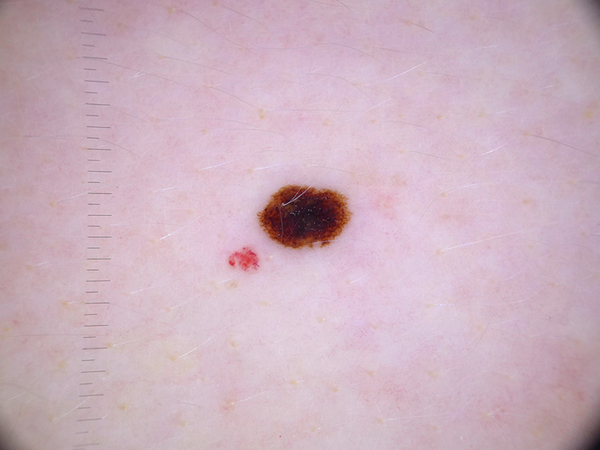
\includegraphics[width=0.23\linewidth]{mel_1.jpg} &
%		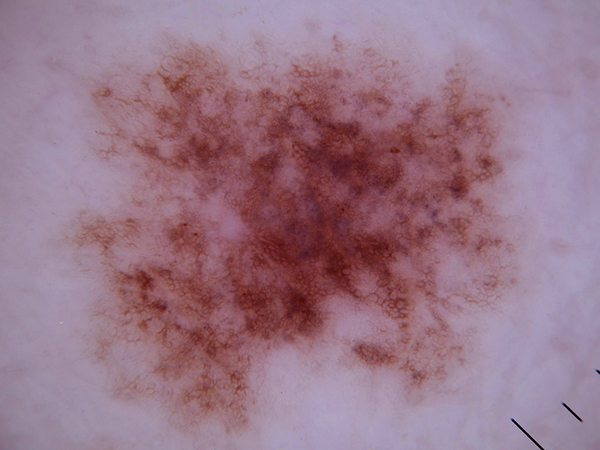
\includegraphics[width=0.23\linewidth]{mel_2.jpg} &
%		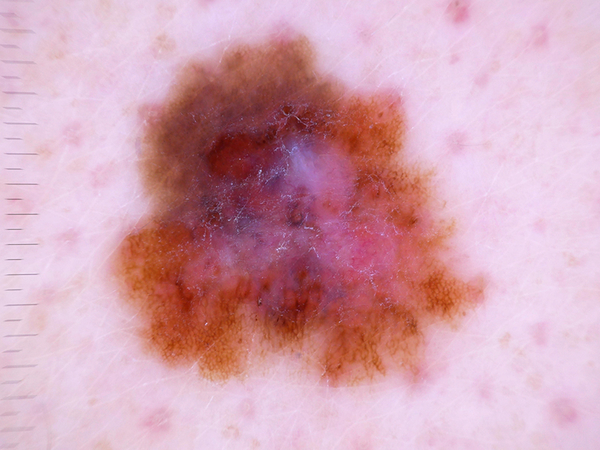
\includegraphics[width=0.23\linewidth]{mel_3.jpg} &
%		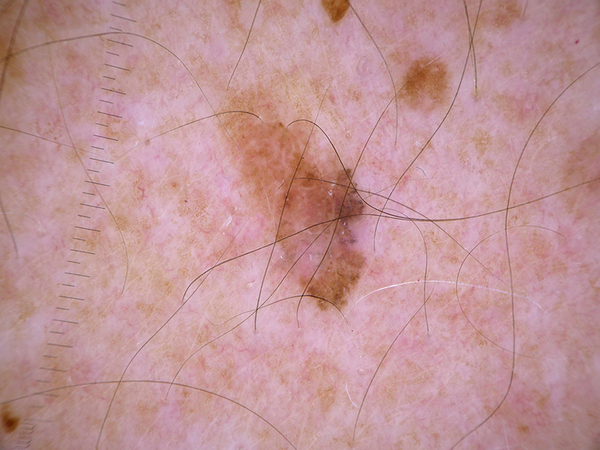
\includegraphics[width=0.23\linewidth]{mel_4.jpg} \\[-1pt]
%		
%		{\scriptsize MEL} &
%		{\scriptsize MEL} &
%		{\scriptsize MEL} &
%		{\scriptsize MEL} \\[6pt]
%		
%		\multicolumn{4}{c}{(b) Inter-class similarity across different lesion categories} \\[2pt]
%		
%		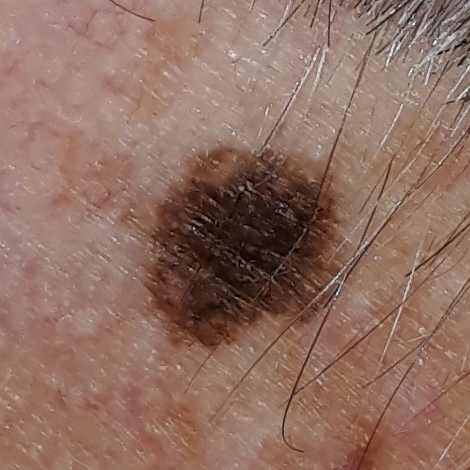
\includegraphics[width=0.23\linewidth]{sim_mel.png} &
%		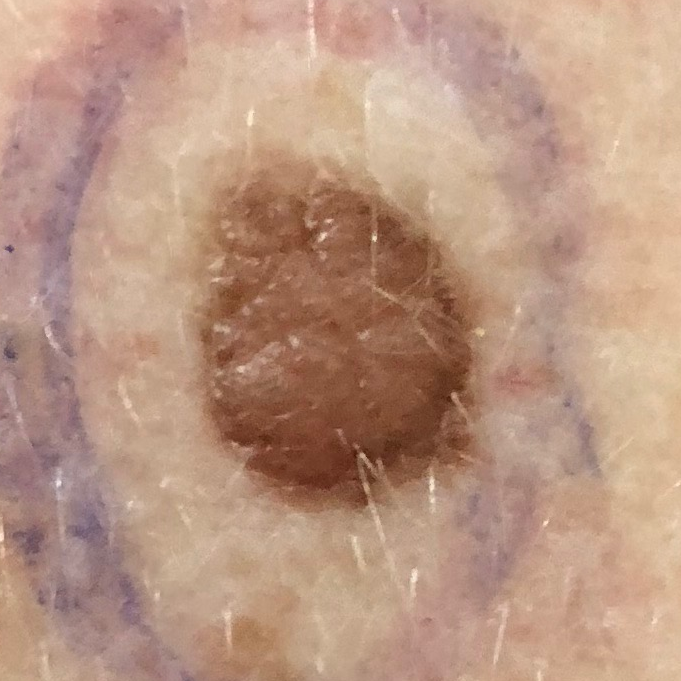
\includegraphics[width=0.23\linewidth]{sim_nev.png} &
%		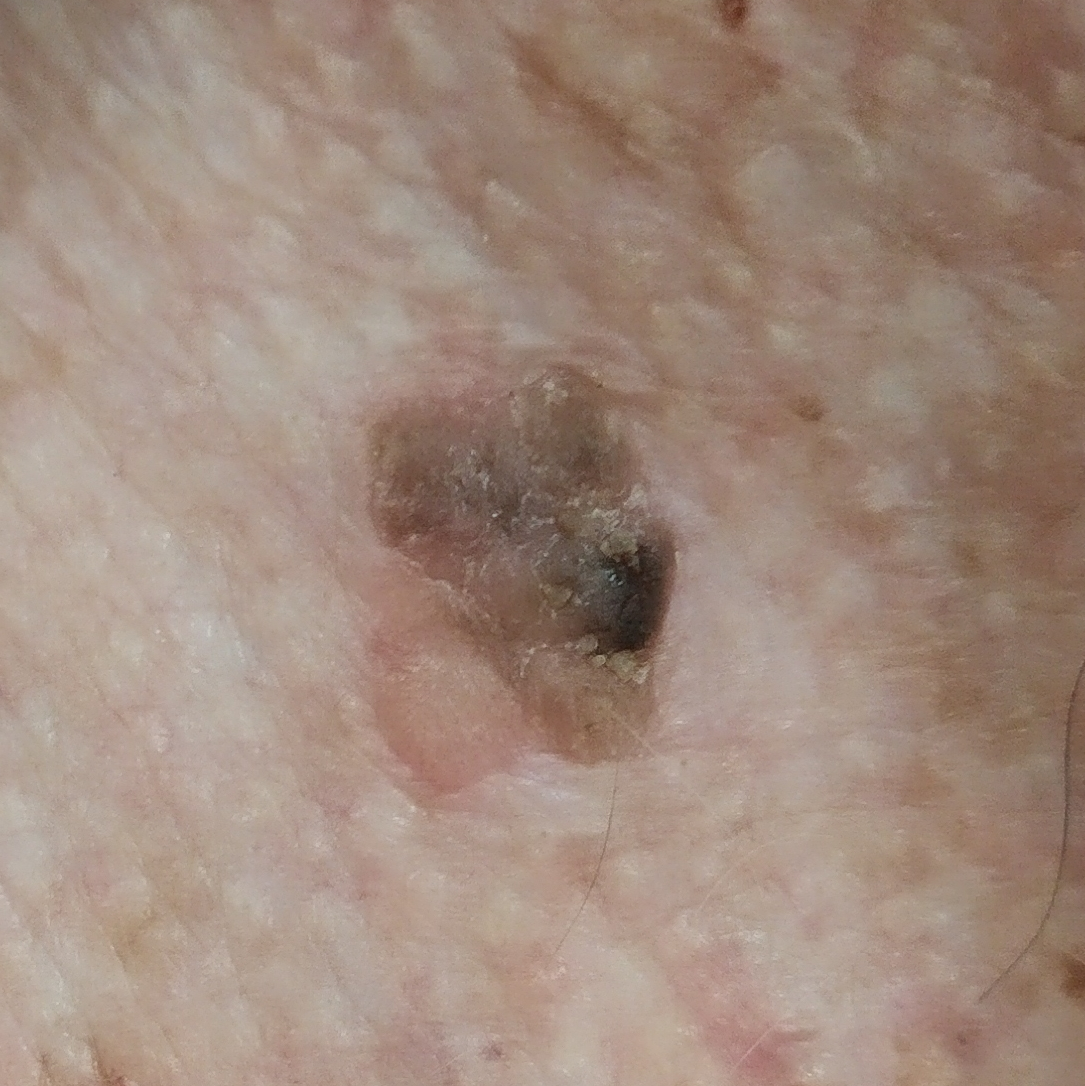
\includegraphics[width=0.23\linewidth]{sim_sek.png} &
%		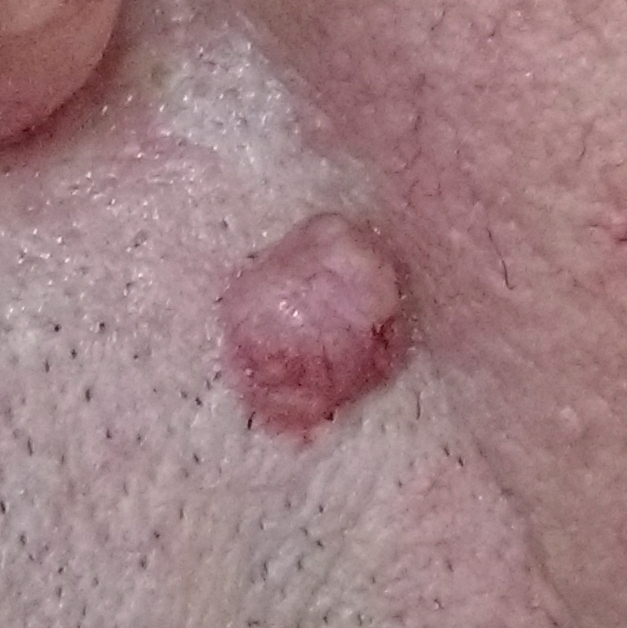
\includegraphics[width=0.23\linewidth]{sim_bcc.png} \\[-1pt]
%		
%		{\scriptsize MEL} &
%		{\scriptsize NEV} &
%		{\scriptsize SEK} &
%		{\scriptsize BCC}
%	\end{tabular}
%	
%	\caption{Representative examples of (a) Intra-class variability within the MEL class and (b) Inter-class similarity across different lesion categories in HAM10000 and PAD-UFES-20.}
%	\label{figure1}
%\end{figure}

\begin{figure}[!ht]
	\centering
	\setlength{\tabcolsep}{2pt}
	\renewcommand{\arraystretch}{0.95}
	
	\begin{tabular}{cccc}
		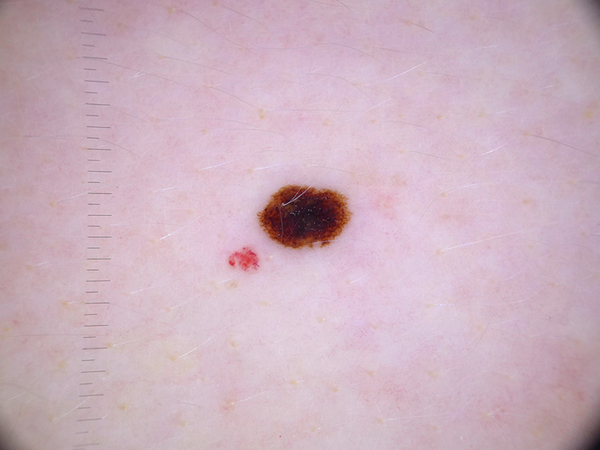
\includegraphics[width=0.23\linewidth]{mel_1.jpg} &
		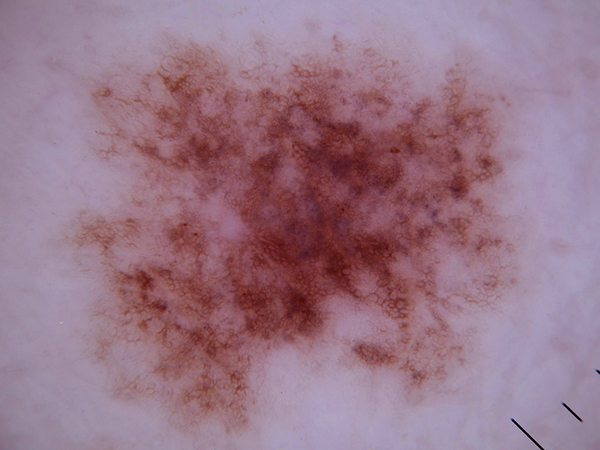
\includegraphics[width=0.23\linewidth]{mel_2.jpg} &
		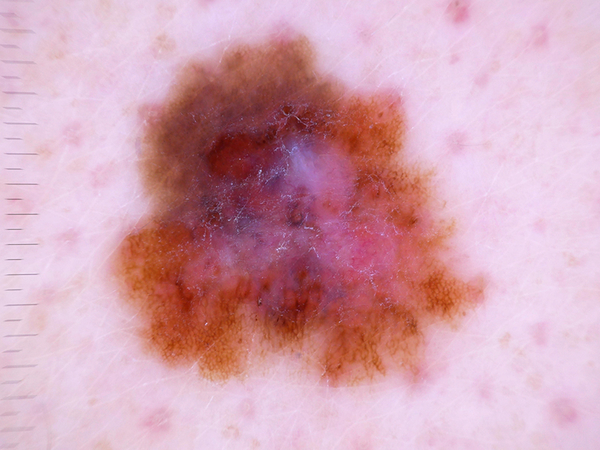
\includegraphics[width=0.23\linewidth]{mel_3.jpg} &
		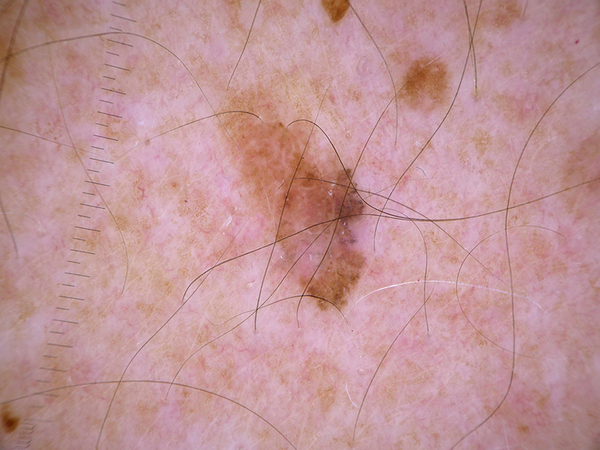
\includegraphics[width=0.23\linewidth]{mel_4.jpg} \\[-1pt]
		
%		{\scriptsize MEL} &
%		{\scriptsize MEL} &
%		{\scriptsize MEL} &
%		{\scriptsize MEL} \\[6pt]
		
		\multicolumn{4}{c}{(a)} \\[10pt]  % 子标签移到图片下方
		
		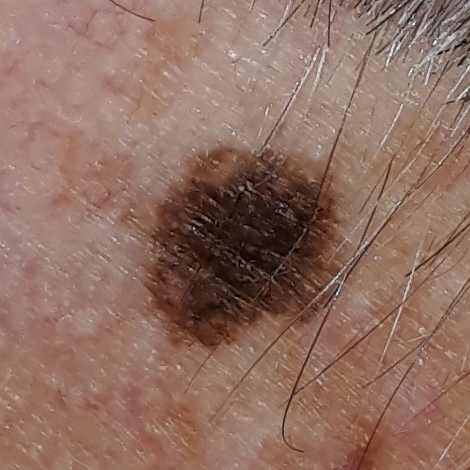
\includegraphics[width=0.23\linewidth]{sim_mel.png} &
		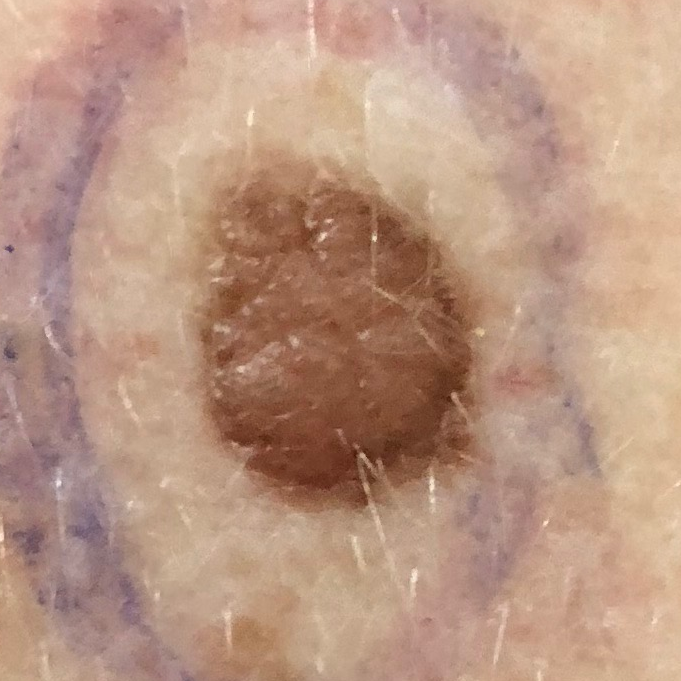
\includegraphics[width=0.23\linewidth]{sim_nev.png} &
		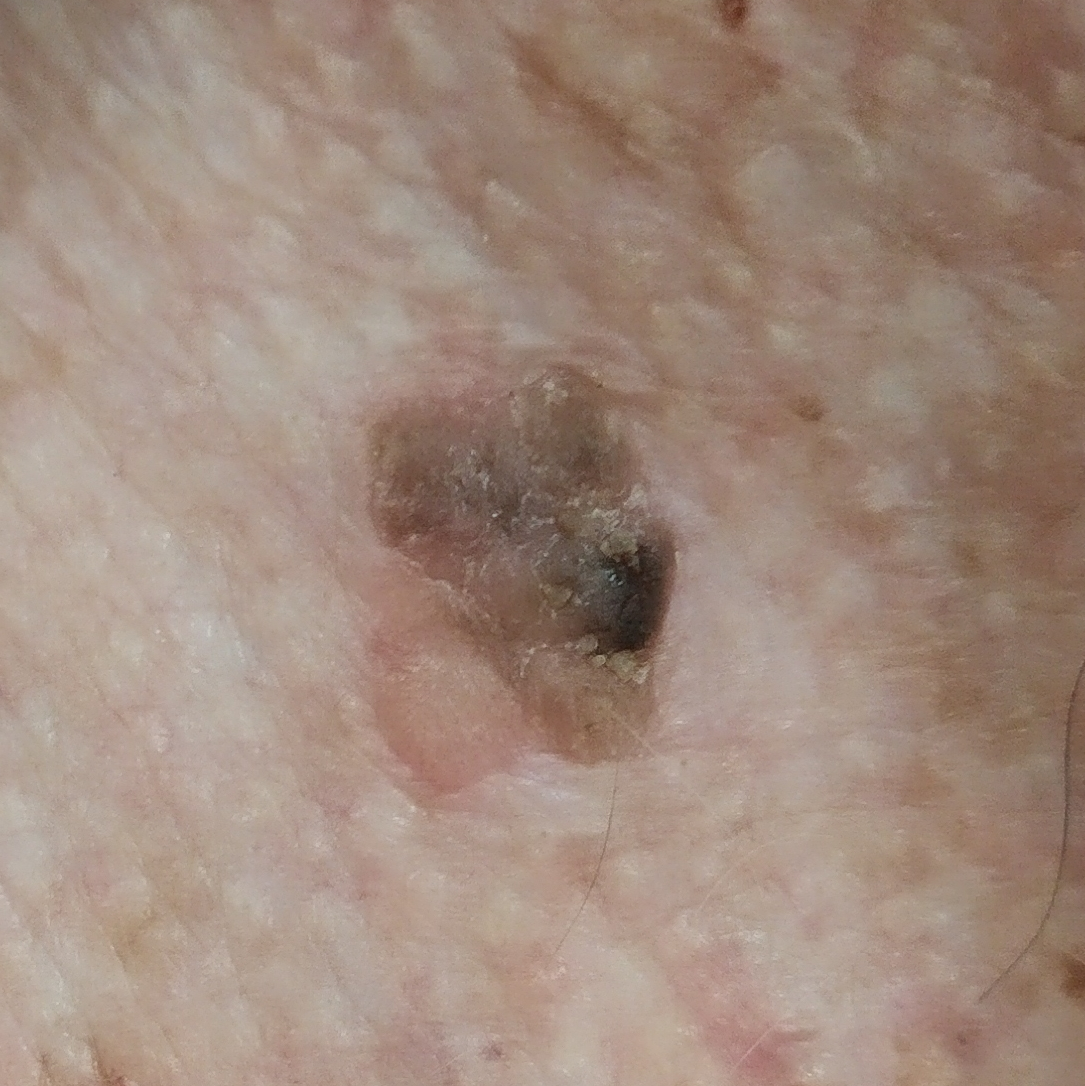
\includegraphics[width=0.23\linewidth]{sim_sek.png} &
		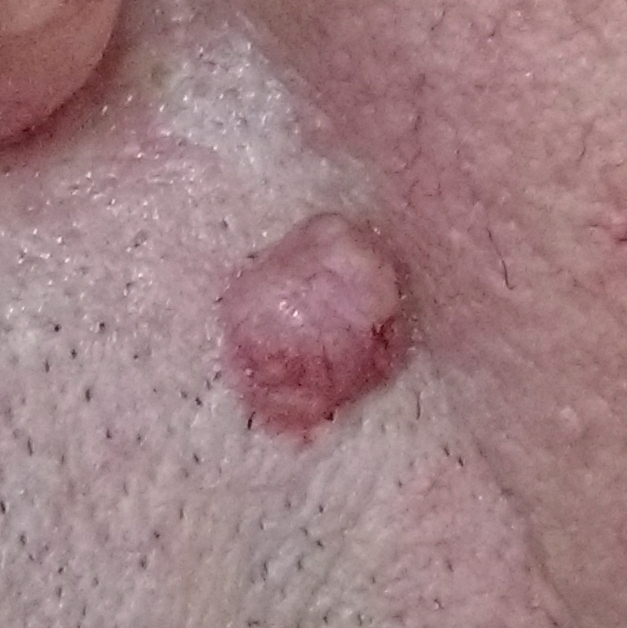
\includegraphics[width=0.23\linewidth]{sim_bcc.png} \\[-1pt]
		
%		{\scriptsize MEL} &
%		{\scriptsize NEV} &
%		{\scriptsize SEK} &
%		{\scriptsize BCC} \\[6pt]
		
		\multicolumn{4}{c}{(b)}
	\end{tabular}
	
	\caption{Examples of (a) intra-class variability within the MEL class and (b) inter-class similarity across the MEL, NEV, SEK, and BCC classes.}
	\label{figure1}
\end{figure}


To address the above limitations, recent studies have introduced clinical metadata into skin lesion classification, showing that imaging data and clinical metadata are complementary when properly fused \cite{pacheco2020impact, khurshid2025multimodal}. Existing fusion methods usually encode metadata as tabular vectors and combine them with visual features through concatenation, feature modulation, or auxiliary-task learning \cite{li2020fusing,pacheco2021attention,khurshid2024optimizing}. Although effective, these task-specific architectures often lack the semantic modeling and transfer ability of medical vision-language models (MVLMs). Moreover, when metadata attributes are strongly correlated with labels, multimodal models may over-rely on textual or tabular cues and ignore essential visual evidence, leading to shortcut learning and unstable predictions \cite{watson2026multimodal}.





MVLMs provide a promising framework for multimodal diagnosis by jointly modeling medical images and textual information. Recent works have adapted vision-language models to dermatology through domain-specific datasets or task-oriented fine-tuning \cite{zhu2026concept,zeng2025mmskin}, and MedGemma provides a medical VLM backbone suitable for downstream clinical tasks \cite{sellergren2025medgemma}. Nevertheless, directly applying generative MVLMs to closed-set skin lesion classification remains challenging. Specifically, full fine-tuning of large-scale models is computationally costly and prone to overfitting on limited medical data. Even with efficient adaptation, open-ended generation may produce invalid labels outside the predefined diagnostic set. More critically, multimodal predictions can suffer from modality bias when textual metadata dominates visual evidence, undermining the model's reliance on clinically essential image features.



To address these challenges, we propose CGVP-MedGemma, a confidence-gated visual prior consistency framework for multimodal closed-set skin lesion classification. The proposed framework adapts an MVLM to integrate lesion images and clinical metadata under an instruction-following paradigm. Instead of treating diagnosis as open-ended text generation, CGVP-MedGemma reformulates it as a constrained closed-set classification task. In addition, an image-only visual prior is introduced during training to encourage the multimodal model to remain grounded in reliable visual evidence, thereby reducing the risk of metadata-induced shortcut learning. This design provides a practical and self-contained multimodal diagnostic scheme, as the visual prior branch operates exclusively during training and is not required at test time.

The main contributions of this study are summarized as follows: 1. We propose an MVLM adaptation framework for multimodal skin lesion classification, which converts structured clinical metadata into natural-language notes and constrains model outputs to predefined diagnostic labels. 2. Building on this, we design a confidence-gated visual prior consistency mechanism, where an independently trained ResNet50-CBAM branch provides image-only soft teacher distributions during training. The teacher-to-student KL regularization encourages the multimodal model to remain aligned with visually supported diagnostic evidence, thereby reducing excessive reliance on clinical textual cues without increasing inference cost. 3. Furthermore, we incorporate class-aware training strategies and 
evaluate the proposed framework on PAD-UFES-20 and HAM10000 datasets \cite{tschandl2018ham10000,pacheco2020padufes20}, demonstrating that CGVP-MedGemma achieves competitive performance against state-of-the-art baselines and provides an effective multimodal diagnostic framework for applying MVLMs to skin lesion classification.


\section{Related works}

\subsection{Skin lesion classification methods}
Early studies treated skin lesion classification as an image classification problem and demonstrated that CNNs can learn discriminative representations directly from clinical and dermoscopic images \cite{esteva2017dermatologist,codella2019skin}. Subsequent works further improved visual feature extraction by introducing deeper network architectures, residual connections, dense blocks, and attention mechanisms \cite{yu2017melanoma,hosny2022refined,wu2020skin}. Representative architectures such as VGG, ResNet, DenseNet, EfficientNet, and MobileNet have been widely adopted as vision-only baselines for skin lesion classification~\cite{simonyan2014very,he2016deep,huang2017densely,tan2019efficientnet,sandler2018mobilenetv2}. These methods have achieved promising results, and in some controlled settings, they have even outperformed dermatologists \cite{brinker2019deep}. However, vision-only classification remains challenging because skin lesions often present high inter-class similarity and substantial intra-class variability. Variations in color, texture, scale, illumination, and acquisition devices may further reduce robustness. Moreover, the inability of visual models to incorporate clinically relevant patient information motivates the development of multimodal diagnostic methods.




\subsection{Metadata fusion methods}
To overcome the limitations of vision-only models, clinical metadata have been explored as an additional information source for skin lesion diagnosis. Such metadata attributes offer complementary diagnostic cues, especially when visual patterns are ambiguous. Pacheco et al.~demonstrated that incorporating patient clinical information improves automated skin cancer detection, underscoring the value of combining lesion images with structured metadata and spurring the development of multimodal fusion methods for dermatology, where metadata is introduced as auxiliary information to enhance vision-based classification~\cite{pacheco2020impact}. 


Existing metadata fusion methods can be grouped into several categories. The simplest method is concatenation, which directly combines image features with encoded metadata features before classification~\cite{pacheco2020impact}. More advanced methods attempt to use metadata to guide or modulate visual representations. For example, MetaNet fuses dermoscopic images and metadata by learning metadata-aware feature representations~\cite{li2020fusing}, while MetaBlock introduces an attention-based mechanism to combine image features and patient information more effectively~\cite{pacheco2021attention}. AuxNet improves multimodal skin lesion classification through auxiliary task learning~\cite{khurshid2024optimizing}. DualRefNet further enhances performance via a dual-stage feature refinement strategy~\cite{khurshid2025multimodal}. These methods demonstrate that clinical metadata can consistently benefit skin lesion classification when properly integrated with visual features.

However, most existing fusion methods represent metadata as fixed tabular vectors and integrate them through task-specific network modules. Such designs may have limited ability to exploit the semantic structure of clinical descriptions and are less flexible than language-based multimodal modeling. More importantly, when certain metadata attributes are highly correlated with specific diagnostic labels, multimodal models may over-rely on non-visual cues and neglect critical visual evidence from lesion images. 


\subsection{MVLM-based methods}

Vision-language models (VLMs) have recently become an important direction in medical image analysis because they can jointly process visual inputs and textual information within a unified representation space. General image-text pretraining methods, such as CLIP, have shown that contrastive learning on large-scale image-text pairs can produce transferable multimodal representations~\cite{radford2021learning}. Inspired by this line of work, several MVLMs have been proposed for clinical image understanding. MedCLIP adapts contrastive vision-language learning to medical images and reports, aiming to learn medical image-text representations with improved data efficiency~\cite{wang2022medclip}. BiomedCLIP further extends biomedical vision-language pretraining by using large-scale biomedical image-text pairs collected from scientific literature~\cite{zhang2023biomedclip}. These studies establish transferable multimodal representations that lay the groundwork for applying vision-language learning to medical image analysis.


In addition to contrastive pretraining, instruction-following medical VLMs have also been explored. LLaVA-Med extends multimodal instruction tuning to biomedical scenarios and enables open-ended medical visual question answering and vision-based dialogue~\cite{li2023llavamed}. MedGemma is a more recent MVLM specially designed for downstream clinical tasks, offering strong multimodal representations suitable for medical image analysis~\cite{sellergren2025medgemma}. In dermatology, several studies have focused on constructing domain-specific image-text resources and adapting VLMs to skin lesion analysis. MM-Skin improves dermatology vision-language modeling using image-text data derived from textbooks~\cite{zeng2025mmskin}. Derm1M builds a large-scale dermatology image-text dataset aligned with clinical ontology knowledge and supports dermatology-oriented vision-language representation learning~\cite{yan2025derm1m}. SkinVL explores multimodal foundation modeling for clinical dermatology and has been evaluated on dermatological image understanding tasks~\cite{yan2025multimodal}. 


Despite these advances, directly applying generative MVLMs to closed-set skin lesion classification remains underexplored. Existing approaches either focus on open-ended visual question answering rather than structured classification, or lack mechanisms to prevent the model from over-relying on textual cues at the expense of visual evidence. In this work, we address these limitations by introducing a parameter-efficient fine-tuning strategy combined with a confidence-gated visual prior consistency mechanism.

\section{Method}


\subsection{Overview of the proposed framework}
% TODO: \usepackage{graphicx} required
%\begin{figure}[]
%	\centering
%	
\includegraphics[width=1.0\linewidth]{method2}
%	\caption{}
%	\label{fig:method2}
%\end{figure}


%\begin{figure}[!h]
%	\centering
%	
\includegraphics[width=1.0\linewidth]{method2}
%	\caption{Overview of the proposed CGVP-MedGemma framework.}
%	\label{fig:framework}
%\end{figure}

\begin{figure}[!h]
	\centering
	\begin{subfigure}[b]{1.0\linewidth}
		\centering
		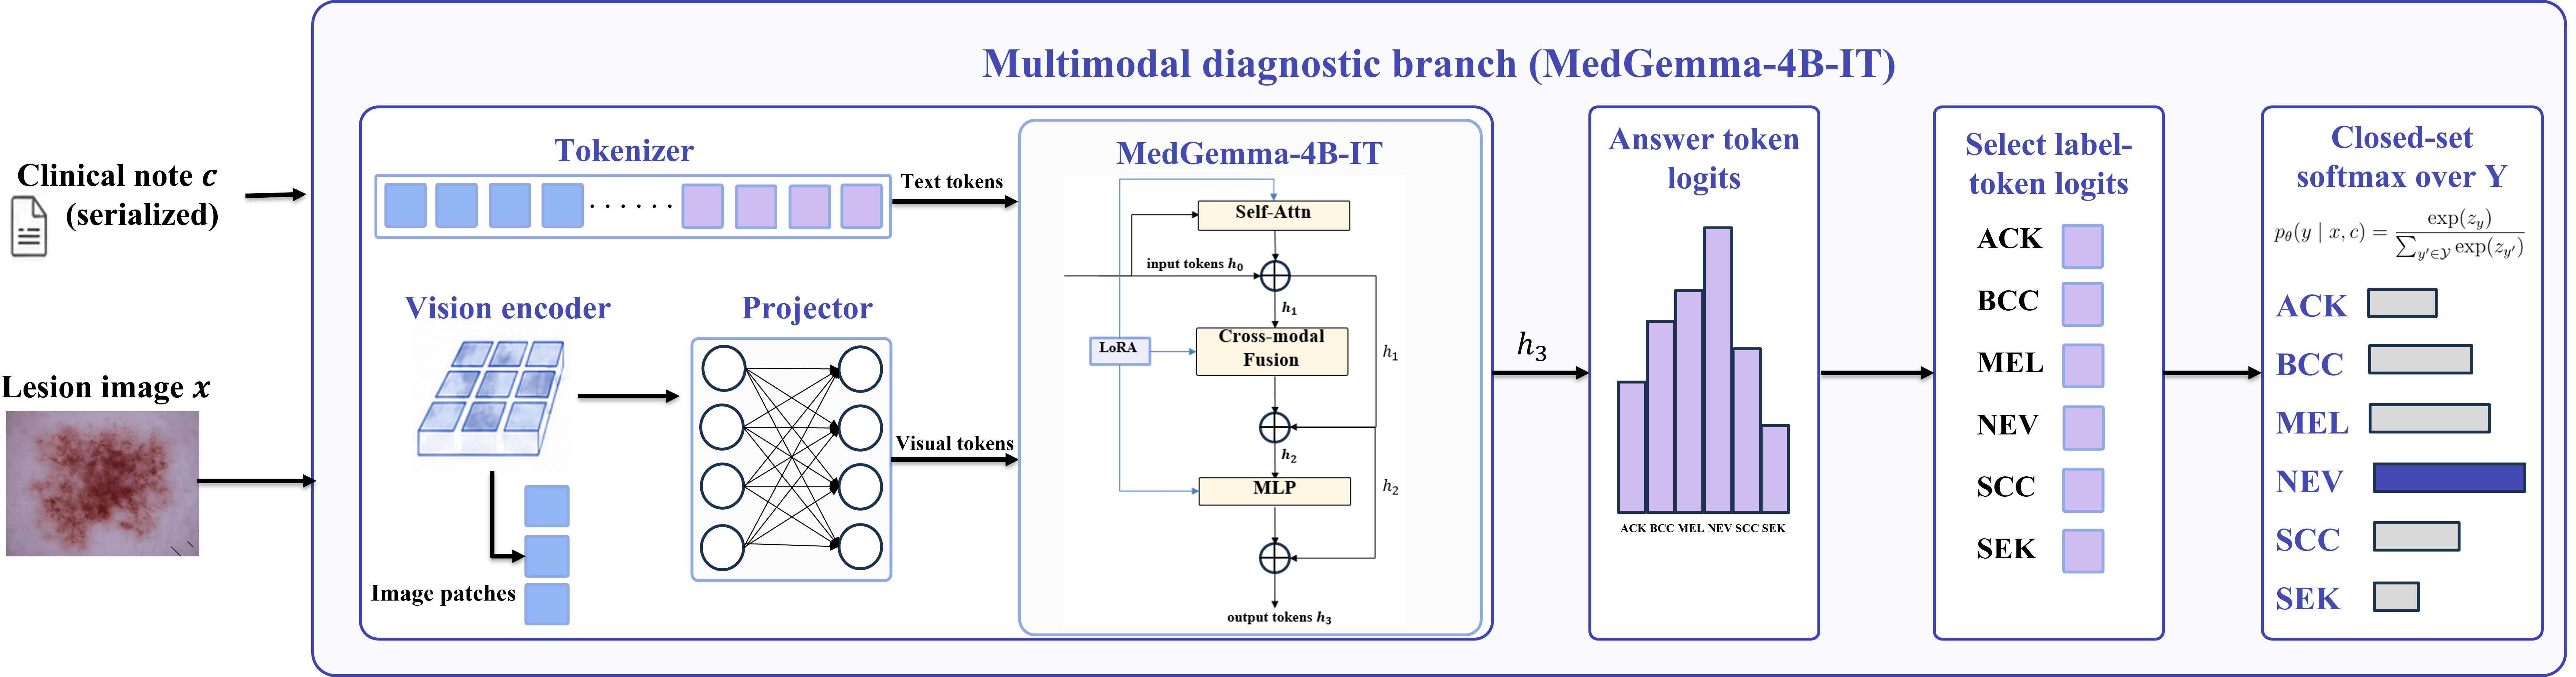
\includegraphics[width=\linewidth]{method}
		\caption{}
		\label{fig:cgvp-medgemma-a}
	\end{subfigure}
	
	\vspace{0.5cm}  % 上下子图间距
	
	\begin{subfigure}[b]{1.0\linewidth}
		\centering
		
\includegraphics[width=\linewidth]{method2}
		\caption{}
		\label{fig:cgvp-medgemma-b}
	\end{subfigure}
	
	\caption{Overview of the proposed CGVP-MedGemma framework. (a) Multimodal diagnostic branch (MedGemma-4B-IT) and (b) visual prior branch.}
	\label{figure2}
\end{figure}

As shown in Figure~\ref{figure2}, the proposed CGVP-MedGemma framework is designed to adapt a generative MVLM for multimodal closed-set skin lesion classification, while explicitly grounding its predictions in visual evidence. It contains a multimodal diagnostic branch and a visual prior branch. The multimodal branch accepts a lesion image alongside serialized clinical metadata as input and processes them through MedGemma-4B-IT under an instruction-following paradigm. By employing LoRA for parameter-efficient adaptation and constraining the model output to a predefined diagnostic label set, the branch effectively converts open-ended generation into closed-set classification.

In parallel, we train an independent ResNet50-CBAM network exclusively on lesion images to generate a vision-based diagnostic distribution. Following pretraining, this visual prior branch is frozen and activated only during the fine-tuning of the main MVLM. Its output serves as a visual reference that is structurally decoupled from clinical metadata. To prevent unreliable visual guidance from affecting ambiguous samples, we introduce a confidence gate: only high-confidence visual prior predictions are used to construct the KL-divergence consistency loss. This regularization encourages the multimodal branch to exploit clinical metadata while avoiding excessive dependence on textual cues. During inference, the visual prior branch is removed, and prediction is performed solely by the LoRA-adapted MedGemma branch. Therefore, the proposed mechanism improves visual consistency during training without introducing additional inference-time cost.


\subsection{Problem formulation}

We formulate skin lesion diagnosis as a multimodal closed-set classification task. Each training sample consists of a lesion image $x \in \mathbb{R}^{H \times W \times 3}$ and its associated clinical metadata $c$, where $c$ comprises 22 structured attributes including personal information, medical history, and lesion morphology. The diagnostic target is a label $y$ drawn from a predefined label set $\mathcal{Y} = \{\text{ACK}, \text{BCC}, \text{MEL}, \text{NEV}, \text{SCC}, \text{SEK}\}$ of 6 categories. The goal is to learn a mapping $f_\theta(x, c) \rightarrow y$ such that the predicted label $\hat{y} = \arg \max p_\theta(y \mid x, c)$ maximizes classification accuracy under conditions of limited training data and severe class imbalance. The model is jointly optimized to exploit visual evidence from $x$ and complementary contextual cues from $c$, while remaining robustly grounded in visual information even when textual cues are strongly predictive.



\subsection{Multimodal input construction}
Rather than encoding clinical metadata as a fixed-dimensional tabular vector, we serialize all 22 attributes in $c$ into a structured natural-language clinical note. More specifically, each attribute is converted into a short descriptive phrase, and the resulting phrases are concatenated into a coherent paragraph. This design preserves the semantic structure of clinical descriptions and allows the language model to leverage its pretrained natural-language understanding capabilities when processing patient-level information. The serialized clinical note is subsequently combined with the lesion image $x$ using an instruction-following prompt template. To prevent the model from exploiting fixed label positions as a spurious shortcut, the ordering of candidate labels within the prompt is randomly shuffled at each training iteration. This prevents the model from learning positional biases and forces it to rely on genuine diagnostic reasoning.

\subsection{Parameter-efficient MVLM adaptation}

\subsubsection{Backbone selection}
We adopt MedGemma-4B-IT as the backbone of the main branch. Unlike general VLMs whose visual encoders are pretrained on natural image-text pairs, MedGemma's visual encoders are pretrained on large-scale medical imaging corpora spanning radiology, pathology, and dermatology~\cite{sellergren2025medgemma}, instilling feature representations that are already sensitive to clinically discriminative patterns such as lesion boundary irregularity and textural heterogeneity. This substantially reduces the domain gap that LoRA fine-tuning must bridge, making adaptation more data-efficient under the small-scale, class-imbalanced conditions of PAD-UFES-20 and HAM10000.


The instruction-tuned variant (-IT) is selected over the base model due to its superior behavioral alignment. Through supervised fine-tuning on medical instruction-following datasets, the -IT variant internalizes a structured response paradigm that naturally maps clinical prompts to concise, well-formed diagnostic outputs. This alignment guarantees consistent task instruction interpretation and constrains generation behavior to the expected answer format, which is a critical requirement in clinical classification scenarios where output predictability and format consistency are essential. With 4 billion parameters, MedGemma-4B-IT further achieves a favorable balance between representational capacity for nuanced multimodal reasoning over complex clinical notes and the parameter efficiency required for effective LoRA-based domain adaptation without catastrophic forgetting of pretrained medical representations.

\subsubsection{Low-rank adaptation}
Full fine-tuning of a 4B model on small-scale clinical datasets is computationally prohibitive and prone to catastrophic forgetting of pretrained representations. 
Therefore, we adopt LoRA, which injects trainable low-rank decomposition matrices into the attention projection layers and feed-forward projections of the transformer~\cite{hu2022lora}. 


The rationale behind using LoRA is that the adaptation from MedGemma-4B-IT to skin lesion classification does not require relearning the entire medical vision-language representation space. Since the backbone has already encoded general medical multimodal knowledge, the downstream task mainly requires a task-specific residual update that adjusts the association among lesion images, serialized clinical metadata, and predefined diagnostic labels. Let $W_0$ denote a pretrained weight matrix and $W^*$ denote the ideal weight. The full fine-tuning update can be expressed as:
\begin{equation}
W^* = W_0 + \Delta W^*
\end{equation}
In this study, $\Delta W^*$ is assumed to be dominated by a limited number of task-specific directions, so it can be approximated by a low-rank residual:
\begin{equation}
\Delta W^* \approx BA, \, A \in \mathbb{R}^{r \times d}, \, B \in \mathbb{R}^{d \times r}, \, r \ll d
\end{equation}
where $r$ is the rank, $d$ is the original weight dimension, and only $A$ and $B$ are updated during training. The effective transformation is therefore:
\begin{equation}
h' = W_{0}h
+\frac{\alpha}{r}BAh
=
\left(
W_{0}+\frac{\alpha}{r}BA
\right)h.
\end{equation}
where $h$ is the input hidden representation and $\alpha$ is the LoRA scaling factor. This means that LoRA preserves the pretrained weight $W_0$ while learning a compact task-specific correction. For the attention module, LoRA changes the effective query, key and value projections as follows:
\begin{equation}
	Q = X \left( W_{Q}^{0} + \Delta W_{Q} \right), \,
	K = X \left( W_{K}^{0} + \Delta W_{K} \right), \,
	V = X \left( W_{V}^{0} + \Delta W_{V} \right).
\end{equation}
Thus, the learned low-rank residuals directly affect how image tokens, clinical text tokens, and answer-position tokens attend to each other. Updates to $Q$ and $K$ modify the matching of multimodal diagnostic cues, while updates to $V$ affect the information propagated to subsequent layers. When applied to feed-forward projections, LoRA further reshapes task-specific hidden representations for closed-set lesion discrimination.

\subsubsection{Closed-set classification head}
A generative VLM produces a probability distribution over the entire vocabulary at each decoding step, treating diagnosis as a sequence generation problem. This formulation introduces two critical problems: (1) The model may generate label strings not in $\mathcal{Y}$, resulting in invalid predictions. (2) Probability mass is spread over many irrelevant tokens, yielding poorly calibrated class-level confidence estimates.


To resolve both issues, we construct a \textbf{closed-set classification head}. At the single answer token position, we extract only the logits $\{z_{y_k}\}_{k=1}^{K}$ corresponding to the $K$ label tokens and renormalize them within $\mathcal{Y}$:
%
\begin{equation}
p_\theta(y_k \mid x, c) = \frac{\exp(z_{y_k})}{\sum_{k'=1}^{K} \exp(z_{y_{k'}})} 
\end{equation}

This converts open-ended generation into a classification problem, eliminates label hallucination, and produces calibrated probability estimates over the diagnostic label set.

\subsubsection{Classification objective}
The classification objective is a label-smoothed weighted cross-entropy:
%
\begin{equation}
	\mathcal{L}_{\mathrm{cls}} 
	= -\sum_{k=1}^{K} w_k \cdot \tilde{y}_k \log p_\theta(y_k \mid x,c)
	\label{eq:cls_loss}
\end{equation}

where \(\tilde{y}_k = (1 - \epsilon) \cdot 1[y = y_k] + \epsilon / K\) is the label-smoothed soft target with smoothing factor \(\epsilon\), and \(w_k\) is a class-specific weight computed as the normalized inverse square root of class frequency:

\begin{equation}
	w_k = \frac{1 / \sqrt{n_k}}{\sum_{k'=1}^K 1 / \sqrt{n_{k'}}} 
\end{equation}

where \(n_k\) is the number of training samples in class \(k\). This reweighting scheme alleviates the adverse effects of long-tailed class distributions by upweighting rare categories without the extreme sensitivity associated with inverse-frequency weighting.


\subsection{Confidence-gated visual prior consistency}
In small-scale and class-imbalanced clinical datasets, certain metadata attributes can be highly correlated with specific diagnostic labels. Under such conditions, the multimodal model is prone to learning metadata-driven shortcuts, thereby effectively ignoring the visual content of $x$. This over-reliance on textual cues leads to fragile predictions that tend to fail when metadata quality is degraded or incomplete.

To counteract this tendency, we introduce an independent visual prior branch that provides a purely vision-based reference distribution and impose a consistency constraint that penalizes excessive divergence of the main model's multimodal output from this visual reference.

\subsubsection{Visual prior branch architecture}
This visual prior branch adopts a ResNet50 as the backbone augmented with a Convolutional Block Attention
Module (CBAM) \cite{woo2018cbam} inserted after the final residual stage. CBAM applies sequential channel attention and spatial attention to the extracted feature maps: channel attention selectively reweights feature channels according to their discriminative relevance to lesion recognition, while spatial attention directs the model's receptive field toward lesion-informative spatial regions. This combination strengthens the branch's ability to extract diagnostically meaningful features from lesion images, independent of any textual content. 


The visual prior branch is trained independently on image-label pairs using a class-balanced Focal Loss~\cite{lin2017focal} combined with a weighted random sampler to handle long-tailed class distributions, where the loss is defined as:
\begin{equation}
	\mathcal{L}_{\text{vis}} = -\sum_{k=1}^{K} w_k \cdot (1 - p_r(y_k \mid x))^{\gamma} \log p_r(y_k \mid x) 
\end{equation}
where $w_k$ denotes the class-specific weight, $\gamma$ is the focusing parameter. After training, all parameters of this branch are frozen for all subsequent stages. Crucially, the branch takes only $x$ as input and has no access to $c$, ensuring that its output distribution $p_r(y \mid x)$ constitutes a structurally pure visual diagnostic reference, free from any form of textual shortcut.



\subsubsection{Confidence-gated consistency regularization}
With the frozen visual prior providing a reliable vision-based reference, we introduce a consistency regularization mechanism that encourages the main model's multimodal predictions to remain grounded in visual evidence. However, not all training samples yield reliable predictions from the visual prior branch. For visually ambiguous samples, enforcing consistency with an uncertain prior could introduce harmful gradient noise and destabilize training. We therefore apply a confidence gate that restricts regularization to samples for which the visual prior is sufficiently certain. The visual prior branch produces an image-only probability distribution $p_r(y \mid x_i)$. The high-confidence sample set is therefore defined according to the maximum probability of the image-only distribution: \begin{equation}
	\mathcal{G} = \{\, i \mid \max_{y \in \mathcal{Y}} p_r(y \mid x_i) > \tau \,\},
	\label{eq:gated_set}
\end{equation}
where $\tau$ is a confidence threshold. For samples in $\mathcal{G}$, the frozen visual prior is treated as a soft teacher distribution, and a KL divergence penalty is imposed to align the multimodal prediction $p_\theta(y \mid x_i,c_i)$ with the frozen visual reference $p_r(y \mid x_i)$:
\begin{equation}
	\mathcal{L}_{\mathrm{KL}} =
	\frac{1}{|\mathcal{G}| + \epsilon}
	\sum_{i \in \mathcal{G}}
	D_{KL}\!\left(
	p_r(y \mid x_i)\,\|\,p_{\theta}(y \mid x_i, c_i)
	\right),
	\label{eq:kl_gated}
\end{equation}
where $\epsilon$ is a constant for numerical stability. Since $p_r$ is produced by the frozen visual prior branch, gradients flow only through the multimodal prediction $p_\theta$. In this formulation, the visual prior branch serves as a soft teacher that encourages the main model to assign sufficient probability mass to visually supported diagnostic categories. Importantly, $p_r(y \mid x)$ is not injected into the input prompt or intermediate features of the main model. Therefore, the visual prior acts only as a consistency constraint and does not replace multimodal reasoning or introduce additional inference-time cost. The overall training objective combines the classification loss with the consistency regularization:
%
\begin{equation}
	\mathcal{L} = \mathcal{L}_{\mathrm{cls}} + \lambda\, \mathcal{L}_{\mathrm{KL}}
	\label{eq:total_loss}
\end{equation}
%
where $\lambda$ controls the relative strength of visual consistency regularization. The visual prior branch is active only during training. As a result, the proposed mechanism adds no inference-time computational cost.




%\subsection{Training strategy}

%Our experiment is conducted on NVIDIA RTX 4090 24GB GPU with the public PAD-UFES-20 dataset for training and validation. The dataset is split at the patient level to prevent data leakage. To evaluate generalization performance, we additionally adopt the ISIC 2019 dataset as an external test set.

%The visual prior branch adopts an ImageNet-pretrained ResNet50 with an input resolution of $320 \times 320$. To mitigate class imbalance, we employ weighted random sampling and Focal Loss ($\gamma$ = 1.5), optimizing the model with AdamW and a ReduceLROnPlateau scheduler. This branch is trained for $30$ epochs, and then its parameters are frozen for subsequent fine-tuning.
%
%For the main model, we apply LoRA fine-tuning using bfloat16 precision (rank = 32, $\alpha$ = 64, dropout = 0.05). Training lasts for 15 epochs with a global batch size of 4. We adopt a cosine learning rate schedule with warmup (initial $5\times10^{-5}$, warmup ratio 0.1) and set the gradient clipping threshold to 0.5. The loss is computed only at the answer token positions. The regularization weight $\lambda$ and the confidence gate threshold $\tau$ are set to 0.05 and 0.85, respectively, which are determined through ablation studies on the validation set.


%For optimization, the model is trained for 5 epochs, with both the per-device training batch size and evaluation batch size set to 1. Gradient accumulation over 8 steps is adopted to increase the effective batch size. The initial learning rate is set to \(5\times10^{-5}\), the learning rate scheduler follows a cosine schedule, the warmup ratio is set to 0.1, and the maximum gradient norm is set to 0.5. To make the generative model more stable for closed-set classification, the supervision loss is computed only on the label token at the answer position, while the prompt tokens and padding tokens are excluded from loss calculation. In addition, the label order in the prompt is randomly shuffled during training to reduce potential positional bias. The main classification objective is a cross-entropy loss with class weights and label smoothing. The class weights are constructed from the inverse square root of class frequencies in the training set and are further normalized to alleviate class imbalance. When consistency learning is enabled, a KL-divergence-based regularization term is added to the main classification loss, with its weight set to 0.05. This consistency constraint is activated only when the maximum class probability from the auxiliary visual prior branch exceeds 0.85, so as to avoid the negative effect of low-confidence priors.

\section{Experiments}

\subsection{Datasets}


We evaluate the proposed framework on PAD-UFES-20 and HAM10000 \cite{tschandl2018ham10000,pacheco2020padufes20}. The class distribution of the datasets are shown in Table~\ref{table1}.
\begin{table*}[!htbp]
	\centering
	\renewcommand{\arraystretch}{1.15}
	\caption{Class distribution of PAD-UFES-20 and HAM10000.}
	\vspace{1pt}
	\setlength{\tabcolsep}{4pt}
	\small
	\resizebox{\textwidth}{!}{%
		\begin{tabular}{l|c|c|c|c|c|c|c|c|c}
			\hline
			\diagbox[width=9em,height=2\baselineskip]{\textbf{Dataset}}{\textbf{Class}} 
			& \textbf{ACK} 
			& \textbf{BCC} 
			& \textbf{MEL} 
			& \textbf{NEV} 
			& \textbf{SCC} 
			& \textbf{SEK} 
			& \textbf{DF} 
			& \textbf{VASC} 
			& \textbf{Total} \\
			\hline
			\textbf{PAD-UFES-20~\cite{pacheco2020padufes20}} 
			& 730 
			& 845 
			& 52 
			& 244 
			& 192 
			& 235 
			& -- 
			& -- 
			& 2,298 \\
			\hline
			\textbf{HAM10000~\cite{tschandl2018ham10000}} 
			& 327 
			& 514 
			& 1,113 
			& 6,705 
			& -- 
			& 1,099 
			& 115 
			& 142 
			& 10,015 \\
			\hline
		\end{tabular}%
	}
	
	\vspace{3pt}
	\begin{minipage}{0.98\textwidth}
		\footnotesize
		\textit{Note:} In HAM10000, AKIEC corresponds to ACK, NV corresponds to NEV, and BKL corresponds to SEK in this aligned class distribution.
	\end{minipage}
	\label{table1}
\end{table*}

PAD-UFES-20 contains 2298 clinical images captured by smartphones and structured patient metadata across six skin lesion classes: actinic keratosis (ACK), basal cell carcinoma (BCC), melanoma (MEL), melanocytic nevus (NEV), squamous cell carcinoma (SCC), and seborrheic keratosis (SEK). HAM10000 consists of 10,015 dermoscopic images collected from multiple institutions and covers seven diagnostic categories. In this study, HAM10000 is used for direct cross-dataset evaluation. Specifically, the model is first trained on PAD-UFES-20 and then directly tested on HAM10000 without additional fine-tuning, so that the transferability of the learned multimodal diagnostic model can be assessed. Since HAM10000 does not contain the SCC category and the DF and VASC categories have no counterparts in PAD-UFES-20, we retain the shared categories ACK, BCC, MEL, NEV, and SEK and exclude DF and VASC from evaluation. Therefore, HAM10000 results are reported on a mapped five-category label space, while PAD-UFES-20 remains the primary six-category multimodal training dataset.



\subsection{Evaluation metrics}
We evaluate model performance using three complementary metrics: Accuracy (ACC), Recall, and Balanced accuracy (BACC). Given $N$ total test samples and $M$ diagnostic categories, these metrics are formally defined as: 
\begin{equation}
	Accuracy = \frac{1}{N} \sum_{i=1}^{N} \mathbf{1}(\hat{y}_i = y_i)
\end{equation}

\begin{equation}
	Recall_j = \frac{TP_j}{TP_j + FN_j}
\end{equation}

\begin{equation}
	Balanced\ Accuracy = \frac{1}{M} \sum_{j=1}^{M} Recall_j
\end{equation}


where $TP_j$ and $FN_j$ denote the true positives and false negatives for class $j$, respectively. While ACC provides an overall measure of classification correctness, it can be misleading under class imbalance, as a model that predominantly predicts majority classes may achieve deceptively high accuracy. BACC addresses this by computing the unweighted mean of per-class recall, treating each category equally regardless of its prevalence. 



\subsection{Experimental setup}
\label{4.3}
To prevent data leakage, we split PAD-UFES-20 at the \textbf{patient level} into training (70\%), validation (15\%), and test (15\%) sets. To simulate a real-world clinical environment, we neither impute missing data nor remove samples with missing fields, and we do not employ neural networks for missing value prediction, as any form of imputation would introduce bias~\cite{vo2026explainability,ryan2025does,el2026moving}.


The visual prior branch is initialized with ImageNet-pretrained weights and trained with an input resolution of 320 $\times$ 320. The branch is optimized using AdamW with a ReduceLROnPlateau learning rate scheduler and trained for 30 epochs. Upon convergence, all branch parameters are frozen and remain fixed throughout all subsequent stages.


LoRA fine-tuning of MedGemma-4B-IT is applied exclusively to all 34 transformer decoder blocks of its language model and conducted in bfloat16 precision with rank $r = 32$, scaling factor $\alpha = 64$, and dropout rate 0.05. Training runs for 15 epochs with a global batch size of 4, using a cosine learning rate schedule with linear warmup: initial learning rate $5 \times 10^{-5}$ and warmup ratio 0.1. Gradient clipping is applied with a maximum norm of 0.5. The label smoothing factor $\epsilon$ is set to 0.05. The classification loss and KL divergence regularization are computed exclusively at the answer token position, with all prompt tokens masked from loss computation. The regularization weight $\lambda$ and confidence gate threshold $\tau$ are set to 0.05 and 0.85, respectively. All reported results are averaged over three independent runs with different random seeds to reduce variance. 

\subsection{Visual prior branch configuration}
To identify the optimal backbone for the visual prior branch, we conduct a systematic comparison of five representative CNN architectures~\cite{simonyan2014very,he2016deep,tan2019efficientnet,sandler2018mobilenetv2,huang2017densely} on PAD-UFES-20, evaluating six fusion strategies~\cite{pacheco2020impact,khurshid2025multimodal,li2020fusing,pacheco2021attention,khurshid2024optimizing} under both vision-only and multimodal fusion settings for each backbone. Results are shown in Table~\ref{table2}.


\begin{table*}[!htbp]
	\centering
	\renewcommand{\arraystretch}{1.15}  % 增加行距
	\caption{Performance comparison of five backbones combined with six metadata fusion methods on PAD-UFES-20.}
	\vspace{1pt}
	\setlength{\tabcolsep}{4pt}
	\small
	\resizebox{\textwidth}{!}{%
		\begin{tabular}{l|cc|cc|cc|cc|cc}
			\hline
			\multirow{2}{*}{\diagbox[width=9em,height=2\baselineskip]{\textbf{Method}}{\textbf{Model}}} & \multicolumn{2}{c|}{\textbf{VGG13\cite{simonyan2014very}}} & \multicolumn{2}{c|}{\textbf{ResNet50\cite{he2016deep}}} & \multicolumn{2}{c|}{\textbf{EfficientNet-B4\cite{tan2019efficientnet}}} & \multicolumn{2}{c|}{\textbf{MobileNet-V2\cite{sandler2018mobilenetv2}}} & \multicolumn{2}{c}{\textbf{DenseNet-121\cite{huang2017densely}}} \\
			\cline{2-11}
			& \textbf{ACC} & \textbf{BACC} & \textbf{ACC} & \textbf{BACC} & \textbf{ACC} & \textbf{BACC} & \textbf{ACC} & \textbf{BACC} & \textbf{ACC} & \textbf{BACC} \\
			\hline
			\textbf{Vision-only} & 0.662 & 0.628 & \textbf{0.708} & \textbf{0.657} & 0.678 & 0.643 & 0.669 & 0.649 & 0.680 & 0.665 \\
			\hline
			\textbf{Concat\cite{pacheco2020impact}} & 0.701 & 0.713 & 0.732 & \textbf{0.725} & \textbf{0.735} & 0.708 & 0.712 & 0.717 & 0.722 & 0.720 \\
			\textbf{MetaNet\cite{li2020fusing}} & 0.726 & 0.719 & 0.721 & 0.707 & \textbf{0.729} & 0.705 & 0.708 & 0.703 & 0.724 & \textbf{0.727} \\
			\textbf{MetaBlock\cite{pacheco2021attention}} & 0.728 & 0.736 & \textbf{0.735} & 0.738 & 0.748 & 0.770 & 0.724 & 0.731 & 0.723 & \textbf{0.746} \\
			\textbf{AuxNet\cite{khurshid2024optimizing}} & 0.751 & 0.748 & \textbf{0.757} & \textbf{0.749} & 0.743 & 0.728 & 0.736 & 0.711 & 0.748 & 0.739 \\
			\textbf{DualRefNet\cite{khurshid2025multimodal}} & 0.753 & 0.745 & \textbf{0.759} & 0.748 & 0.751 & 0.738 & 0.746 & 0.724 & 0.756 & \textbf{0.749} \\
			\hline
		\end{tabular}%
	}
	\label{table2}
\end{table*}

Under the vision-only setting, all backbones exhibit a notable gap between ACC and BACC, confirming that class imbalance substantially degrades per-class recognition, particularly for underrepresented categories. Incorporating clinical metadata consistently improves performance across all backbone-fusion combinations. Among vision-only configurations, ResNet50 achieves the best overall performance between ACC and BACC. Based on these results, we select ResNet50 as the backbone of the visual prior branch and further augment it with CBAM to provide a reliable visual reference distribution for the subsequent LoRA fine-tuning stage.


\subsection{Comparison with representative MVLM methods}
We compare CGVP-MedGemma against representative VLMs adapted for dermatology~\cite{li2023llavamed,zeng2025mmskin,yan2025derm1m}. All methods are evaluated on PAD-UFES-20 and HAM10000 following the experimental setup described in Section~\ref{4.3}. Results are summarized in Table~\ref{table3}.

\begin{table}[!htbp]
	\centering
	\renewcommand{\arraystretch}{1.15}
	\caption{Performance comparison of representative MVLMs on PAD-UFES-20 and direct cross-dataset evaluation on the mapped HAM10000 subset.}
	\vspace{1pt}
	\setlength{\tabcolsep}{4pt}
	\small
	\begin{tabular}{l|cc|cc}
		\hline
		\multirow{2}{*}{\diagbox[width=13.5em,height=2\baselineskip]{\textbf{Methods}}{\textbf{Dataset}}} 
		& \multicolumn{2}{c|}{\textbf{HAM10000}} 
		& \multicolumn{2}{c}{\textbf{PAD-UFES-20}} \\
		\cline{2-5}
		& \textbf{ACC} & \textbf{BACC} 
		& \textbf{ACC} & \textbf{BACC} \\
		\hline
		LLaVA-Med-7B\cite{li2023llavamed} 
		& 0.784 & 0.621 & 0.735 & 0.624 \\
		SkinVL-PubMM\cite{zeng2025mmskin} 
		& 0.790 & 0.626 & 0.752 & 0.640 \\
		DermLIP\cite{yan2025derm1m} 
		& \textbf{0.881} & \textbf{0.745} & 0.740 & 0.657 \\
		\textbf{CGVP-MedGemma (Ours)} 
		& 0.787 & 0.661 & \textbf{0.798} & \textbf{0.776} \\
		\hline
	\end{tabular}
	\label{table3}
\end{table}

On PAD-UFES-20, CGVP-MedGemma achieves an ACC of 0.798 and a BACC of 0.776, outperforming all VLM baselines. Our method outperforms LLaVA-Med-7B and SkinVL-PubMM by 0.152 and 0.136 in BACC, respectively, demonstrating that the confidence-gated visual prior consistency mechanism effectively alleviates textual shortcut bias and improves per-class recognition. The gains over multimodal fusion baselines such as DualRefNet further confirm that natural-language serialization of clinical metadata, combined with parameter-efficient VLM adaptation, captures richer semantic clinical context than fixed tabular vector encoding.

On HAM10000, our method achieves an ACC of 0.787 and a BACC of 0.661, which is competitive with LLaVA-Med-7B and SkinVL-PubMM. The gap relative to DermLIP is attributable to DermLIP's use of a million-scale dermatology-specific pretraining dataset~\cite{yan2025derm1m}, which provides substantially richer domain priors than the general medical pretraining of MedGemma. In contrast, our framework targets the practically important scenario of effective adaptation under limited annotated data, without reliance on large-scale domain-specific pretraining resources.


\begin{figure}[!h]
	\centering
	\begin{subfigure}[b]{0.48\linewidth}
		\centering
		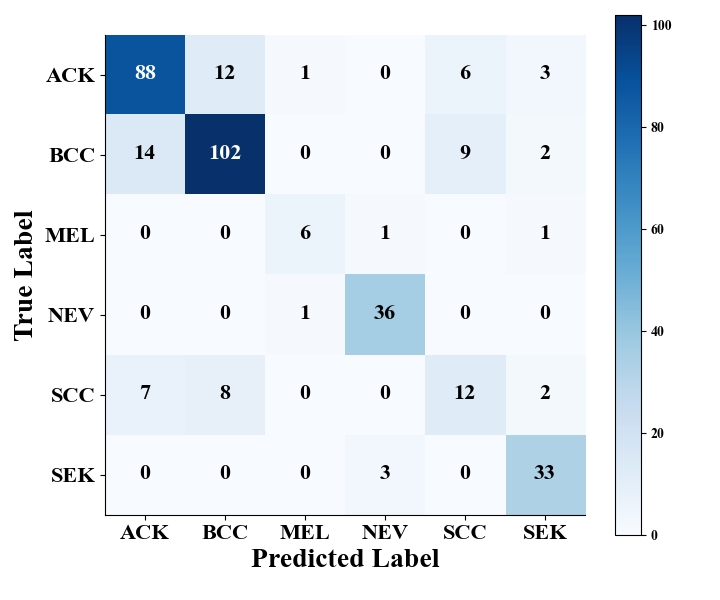
\includegraphics[width=\linewidth]{confusion matrx.png}
		\caption{}
		\label{fig:confusion-matrx-pad}
	\end{subfigure}
	\hfill
	\begin{subfigure}[b]{0.48\linewidth}
		\centering
		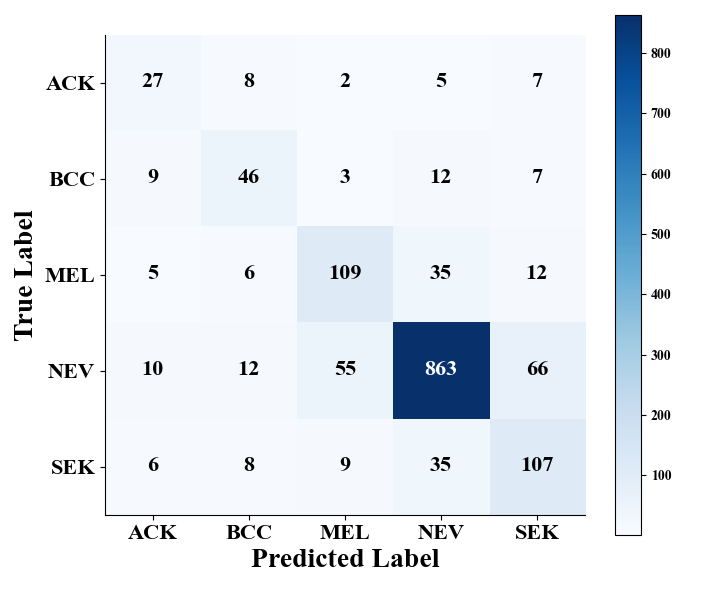
\includegraphics[width=\linewidth]{confusion matrix2.png}
		\caption{}
		\label{fig:confusion-matrx-ham}
	\end{subfigure}
	
	\caption{Confusion matrices of CGVP-MedGemma on (a) PAD-UFES-20 and (b) HAM10000.}
	\label{confusion matrix}
\end{figure}

Figure~\ref{confusion matrix} presents confusion matrices analyzing per-class predictions. On PAD-UFES-20, the model achieves strong recall for ACK (0.800), BCC (0.803), NEV (0.973), and SEK (0.917). MEL attains a recall of 0.750, demonstrating the effectiveness of visual prior guidance for under-represented classes. SCC shows the lowest recall (0.414), mainly confused with ACK and BCC(a clinically justified pattern). On HAM10000, NEV recall is 0.858, with dominant MEL-NEV confusion reflecting dermoscopic similarity. ACK (0.551) and BCC (0.597) exhibit mutual confusion, while SEK (0.648) is mainly misclassified as NEV or ACK. The scarcity of rich textual metadata in HAM10000 limits the model's ability to disambiguate these visually similar lesion pairs; richer visual priors or domain-specific pretraining may benefit minority classes.

 
\subsection{Ablation studies}
\subsubsection{Component-wise ablation}
To quantify the individual contribution of each proposed component, we conduct an incremental ablation study on PAD-UFES-20. Results are shown in Table~\ref{table4}.

\begin{table}[!htbp]
	\centering
	\caption{Step-wise ablation of the training strategy on PAD-UFES-20.}
	\vspace{1pt}
	\label{table4}
	\setlength{\tabcolsep}{15pt}
	\begin{tabular}{lcc}
		\toprule
		\textbf{Training Strategy} & \textbf{ACC} & \textbf{BACC} \\
		\midrule
		MedGemma-4B-IT      & 0.551  & 0.476  \\
		\quad + LoRA fine-tuning           & 0.630  & 0.608  \\
		\quad + Weighted CE loss           & 0.645  & 0.617  \\
		\quad + Ungated visual-prior KL      & 0.751  & 0.738  \\
		\quad \textbf{+ Confidence-gated KL} & \textbf{0.798} & \textbf{0.776} \\
		\bottomrule
	\end{tabular}
\end{table}

The base MedGemma-4B-IT performs poorly, confirming that directly applying a generative MVLM to closed-set skin lesion classification is insufficient. LoRA fine-tuning substantially improves both metrics, demonstrating that parameter-efficient adaptation effectively aligns the pretrained model with the dermatology classification task. Adding weighted cross-entropy loss yields further consistent improvements, confirming that explicit class-frequency reweighting benefits the recognition of underrepresented categories. A substantial gain is observed upon incorporating the visual prior branch, with BACC improving by 0.121 over the weighted CE loss. This gain suggests that the visual prior branch successfully disrupts the main model's over-reliance on metadata shortcuts, thereby stabilizing optimization and enhancing class-level balance. Finally, applying confidence-gated KL regularization further improves both ACC and BACC, achieving the best overall performance. This confirms that selectively enforcing consistency only on high-confidence prior samples is more effective than unconditional regularization, as it avoids propagating unreliable guidance from visually ambiguous samples.

\begin{figure}[!h]
	\centering
	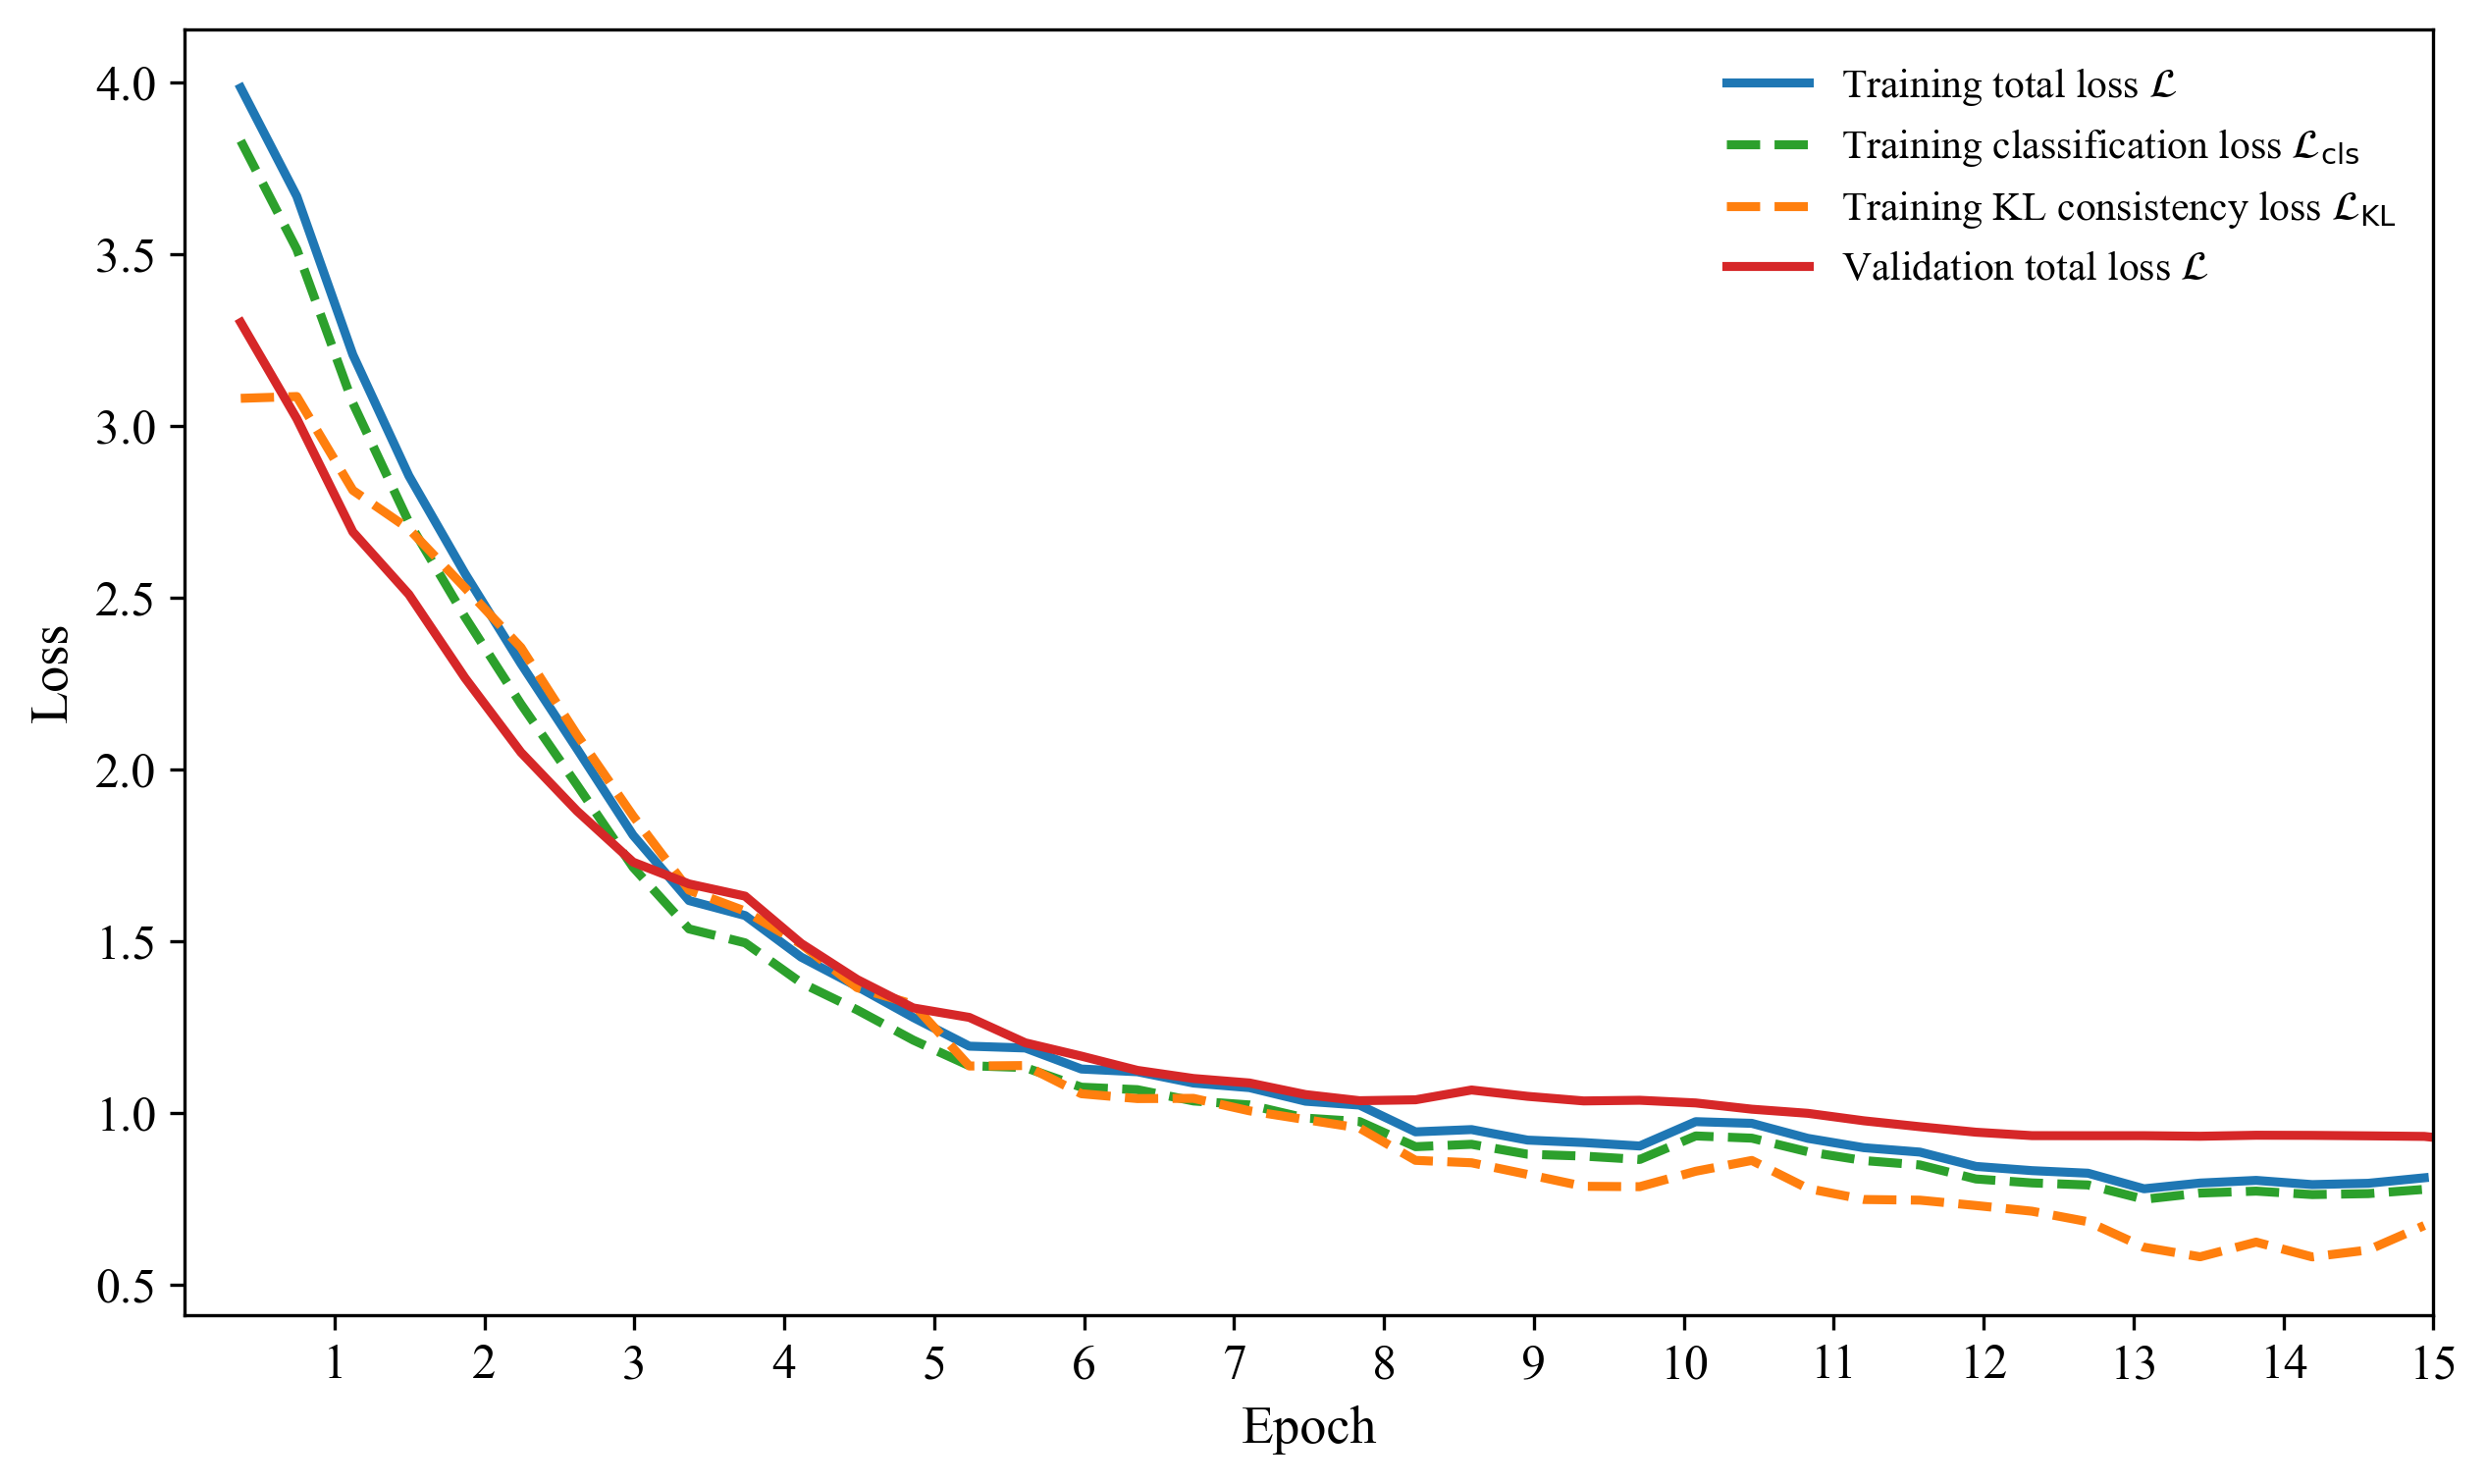
\includegraphics[width=1.0\linewidth]{loss}
	\caption{Training and validation loss curves over 15 epochs on PAD-UFES-20. Training total loss $\mathcal{L}$, classification loss $\mathcal{L}_{cls}$, KL consistency loss $\mathcal{L}_{KL}$, and validation total loss $\mathcal{L}$ are shown.}
	\label{figure4}
\end{figure}
Figure~\ref{figure4} shows the loss curves over 15 epochs. All losses converge by epoch 10, and the small training-validation gap indicates no significant overfitting. $\mathcal{L}_{KL}$ remains consistently lower in magnitude than $\mathcal{L}_{cls}$, as it is computed only over the high-confidence subset $\mathcal{G}$ and scaled by $\lambda = 0.05$. Its stable descent confirms progressive convergence toward visual consistency without destabilizing overall training.
\subsubsection{Clinical metadata ablation}
To assess the contribution of clinical textual information, we evaluate the final model under three metadata configurations: Metadata A comprises 8 commonly available attributes: age, lesion region, itch, grew, hurt, changed, bleed, and elevation. Metadata B extends Metadata A with four additional attributes: gender, Fitzpatrick skin type, and two lesion diameter measurements. Full Metadata includes all available structured attributes in PAD-UFES-20. Following the original dataset setting, missing clinical fields are not imputed or artificially filled with unknown tokens; only available attributes are serialized into the prompt. Results are shown in Table~\ref{table5}.

\begin{table}[!htbp]
	\centering
	\caption{Performance of different metadata on PAD-UFES-20.}
	\label{table5}
	\setlength{\tabcolsep}{15pt}
	\begin{tabular}{lcc}
		\toprule
		\textbf{Metadata Variant} & \textbf{ACC} & \textbf{BACC} \\
		\midrule
		Metadata A           & 0.710  & 0.698  \\
		Metadata B        & 0.752  & 0.747  \\
		\textbf{Full Metadata}             & \textbf{0.798} & \textbf{0.776 } \\
		\bottomrule
	\end{tabular}
\end{table}


Performance improves consistently as richer clinical metadata are provided, with Full Metadata achieving the highest ACC and BACC. This result confirms that the serialized clinical text provides complementary diagnostic information beyond lesion appearance. However, the monotonic benefit of metadata also suggests that the multimodal branch can be strongly influenced by textual clinical cues. Therefore, visual grounding remains necessary when metadata are highly predictive of diagnostic labels. Together with the component-wise ablation in Table~\ref{table4}, these results support the motivation of using an image-only visual prior to constrain the multimodal prediction rather than allowing the model to rely on clinical text alone.


\subsubsection{Qualitative analysis of visual attention}
Figure~\ref{figure5} compares GradCAM attention maps before and after confidence-gated visual prior regularization for four samples. Without the visual consistency constraint, the attention responses are relatively diffuse and partly extend to background regions. After regularization, the activated regions become more concentrated around lesion boundaries and surface texture patterns. This change indicates that the proposed visual prior consistency term encourages the multimodal branch to rely more strongly on lesion-relevant visual evidence, providing complementary evidence to the metadata ablation results.
\begin{figure}[!h]
	\centering
	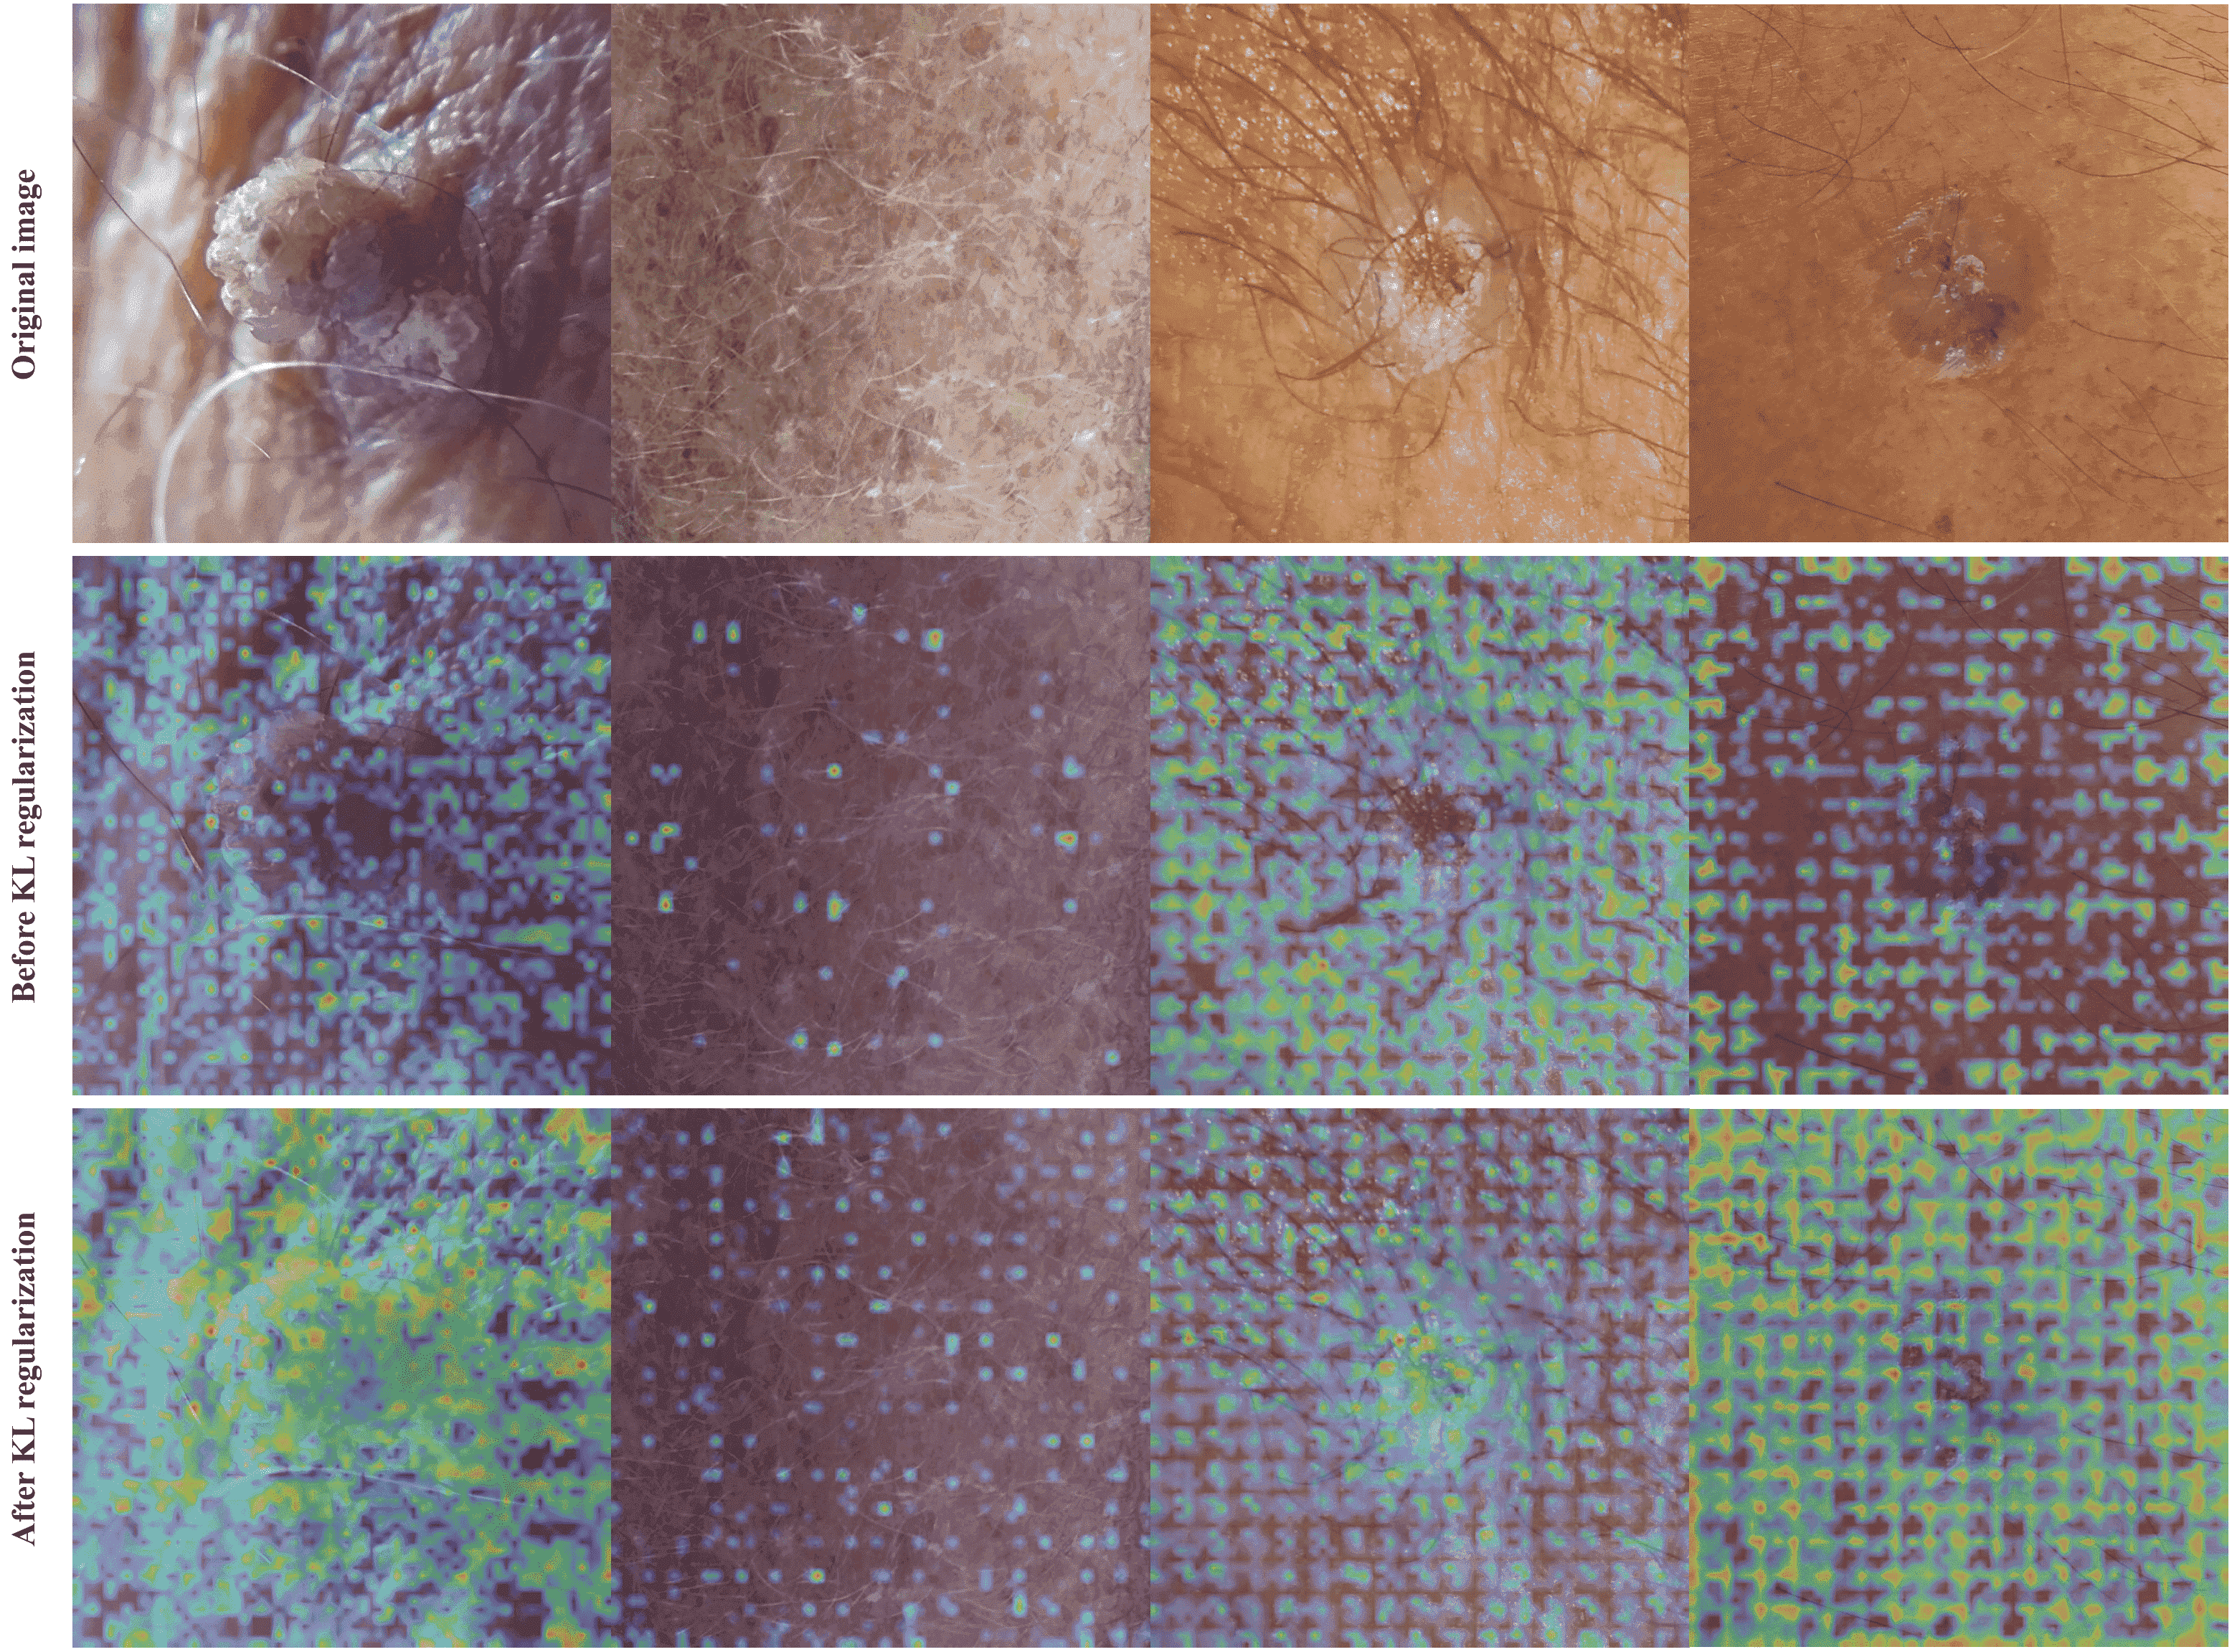
\includegraphics[width=1.0\linewidth]{gradcam}
	\caption{GradCAM attention maps for representative samples from PAD-UFES-20. Row 1: original images. Row 2: attention before KL regularization. Row 3: attention after KL regularization.}
	\label{figure5}
\end{figure}

\subsection{Hyperparameter sensitivity analysis}

Figure~\ref{figure3} reports ACC and BACC across a grid of $\lambda \in [0.00,0.20] $ and $\tau \in [0.70,0.95] $ on PAD-UFES-20. Setting $\lambda = 0$ uniformly degrades both metrics regardless of $\tau$, confirming the contribution of KL regularization. As $\lambda$ increases beyond 0.05, performance declines, indicating over-suppression of textual cues. For $\tau$, excessively low values admit too many ambiguous samples and introduce noisy gradients, while values above 0.90 provide insufficient regularization signal. Performance is relatively stable with $\lambda \in [0.05,0.1]$ and $\tau \in [0.80,0.90]$, justifying the adopted values of $\lambda = 0.05$ and $\tau = 0.85$.
\begin{figure}[!h]
	\centering
	
	\begin{subfigure}[b]{0.48\linewidth}
		\centering
		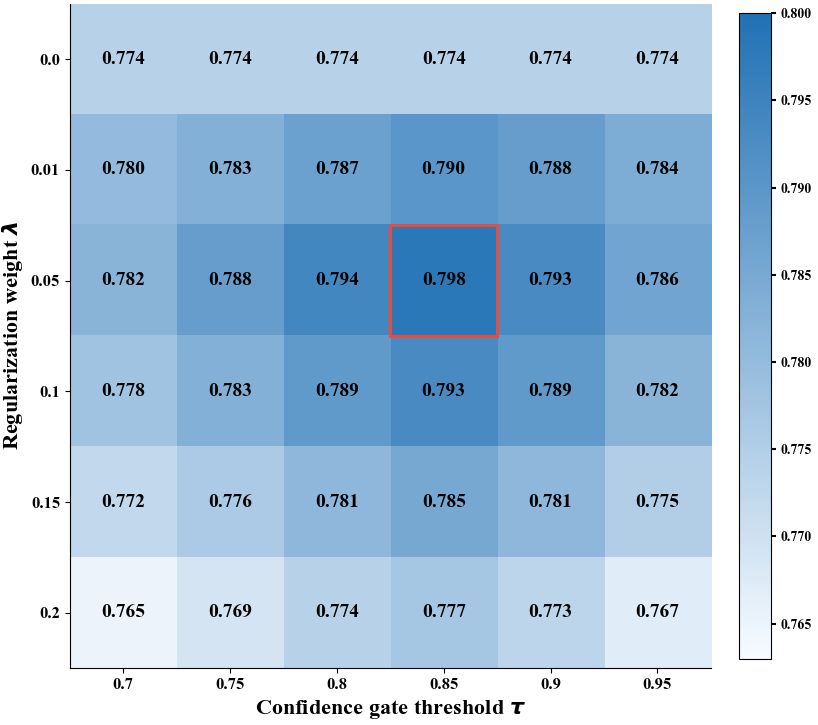
\includegraphics[width=\linewidth]{chaocanshu.png}
		\caption{}
		\label{fig:method3-a}
	\end{subfigure}
	\hfill
	\begin{subfigure}[b]{0.48\linewidth}
		\centering
		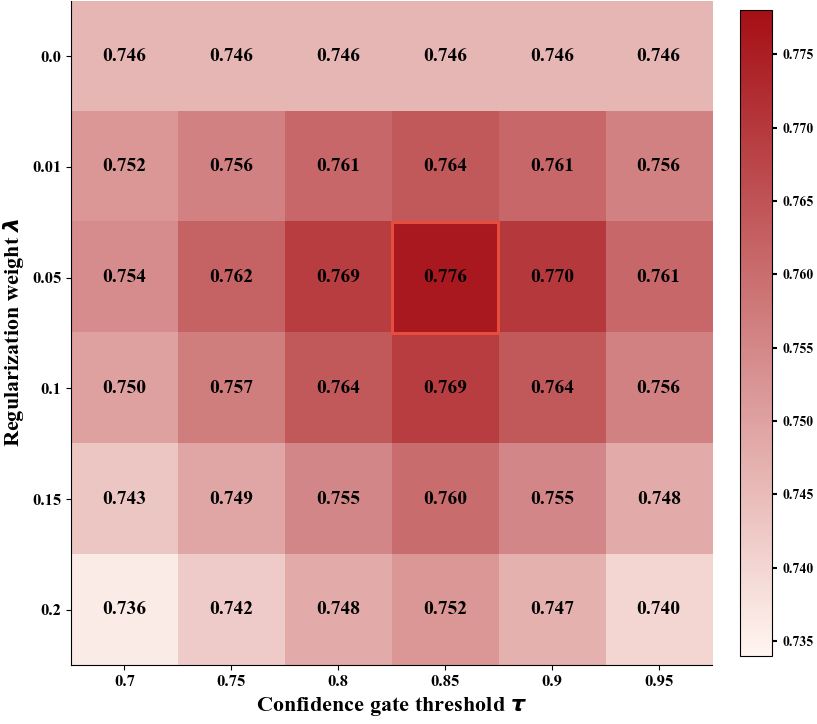
\includegraphics[width=\linewidth]{chaocanshu2.png}
		\caption{}
		\label{fig:method3-b}
	\end{subfigure}
	
	\caption{Sensitivity analysis of regularization weight $\lambda$ and confidence threshold $\tau$ on PAD-UFES-20 in terms of (a) ACC and (b) BACC.}
	\label{figure3}
\end{figure}

\section{Conclusion}

In this paper, we proposed CGVP-MedGemma, a confidence-gated visual prior consistency framework for multimodal closed-set skin lesion classification based on MedGemma-4B-IT. The framework addresses three core challenges in applying generative MVLMs to clinical dermatology: adaptation efficiency under limited data, label hallucination in open-ended generation, and textual shortcut bias induced by metadata-label correlations.

To tackle these challenges, we introduced three complementary components. First, structured clinical metadata is serialized into natural-language notes and combined with lesion images under an instruction-following paradigm, with model outputs constrained to a predefined diagnostic label set via a closed-set classification head, eliminating invalid predictions and improving probability calibration. Second, parameter-efficient LoRA fine-tuning adapts the large pretrained model to the dermatology domain without catastrophic forgetting of medical visual representations. Third, a frozen ResNet50-CBAM visual prior branch provides purely image-based reference distributions, and a confidence-gated KL divergence regularization term penalizes excessive deviation of multimodal predictions from this visual reference, grounding the model in reliable lesion evidence even when textual cues are strongly predictive.


Experiments on PAD-UFES-20 and HAM10000 demonstrate that each component contributes incrementally to the final performance, with the proposed framework achieving competitive results against representative VLM and multimodal fusion baselines. Future work may explore leveraging the generative capacity of the VLM backbone to produce free-text diagnostic rationales alongside classification outputs, further enhancing clinical interpretability.

\section*{CRediT authorship contribution statement}
Ruixi Zhang: Writing --- original draft, Methodology, Visualization, Validation, Software. Dejun Zhang: Investigation, Conceptualization, Data curation. Chen Xiong: Review \& editing, Supervision, Resources, Project administration, Funding acquisition.

\section*{Funding}

This work was supported by the National Key Research and Development Program of China (Grant No. 2024YFB4303400), the Natural Science Foundation of Guangdong Province, China (Grant No. 2025A1515010166), and the Shenzhen Fundamental Research Program, China (Grant No. JCYJ20240813151301003).

\section*{Declaration of competing interest}
The authors declare that they have no known competing financial interests or personal relationships that could have appeared to influence the work reported in this paper.

\section*{Data availability}
The data used in this study are publicly available from the original sources cited in this article. PAD-UFES-20 and HAM10000 can be accessed through the resources described by their original authors.

%\footnote{The code is available at https://github.com/zhangrx59/Graduation-Project.}

\bibliographystyle{elsarticle-num}
\bibliography{main}
\end{document}
